\documentclass[aspectratio=169,10pt]{beamer}

% Theme and colors matching course materials
\usetheme{Madrid}
\usecolortheme{seahorse}

% Enhanced packages for mathematical rigor
\usepackage{amsmath,amssymb,amsfonts}
\usepackage{graphicx}
\usepackage{booktabs}
\usepackage{xcolor}
\usepackage{tikz}
\usepackage{algorithm2e}

% Professional formatting
\setbeamertemplate{navigation symbols}{}
\setbeamertemplate{footline}[frame number]

% Title information
\title{Image Enhancement in the Frequency Domain}
\subtitle{CMSC 178IP - Comprehensive Study Guide}
\author{Digital Image Processing Course}
\institute{Computer Science Department}
\date{\today}

\begin{document}

% Title slide
\begin{frame}
\titlepage
\end{frame}

% Table of contents
\begin{frame}{Course Outline}
\tableofcontents
\end{frame}

\section{Introduction}

\begin{frame}{What is Frequency Domain Enhancement?}
\begin{alertblock}{Definition}
Frequency domain enhancement processes images by transforming them to the frequency domain, applying filters, and transforming back to the spatial domain.
\end{alertblock}

\textbf{Mathematical Foundation:}
$$g(x,y) = \mathcal{F}^{-1}\{H(u,v) \cdot F(u,v)\}$$

Where:
\begin{itemize}
\item $f(x,y)$ = input image
\item $g(x,y)$ = output (enhanced) image
\item $F(u,v) = \mathcal{F}\{f(x,y)\}$ = Fourier transform of input
\item $H(u,v)$ = frequency domain filter
\item $\mathcal{F}^{-1}$ = inverse Fourier transform
\end{itemize}

\textbf{Key Advantages:}
\begin{itemize}
\item Direct frequency manipulation
\item Efficient filtering of periodic noise
\item Theoretical foundation for filter design
\item Insight into image frequency content
\end{itemize}
\end{frame}

\begin{frame}{Problem Setup and Motivation}
\textbf{Why frequency domain enhancement?}

\begin{columns}
\column{0.6\textwidth}
\textbf{Spatial Domain Limitations:}
\begin{itemize}
\item Convolution can be computationally expensive
\item Difficult to remove specific frequency components
\item Limited insight into periodic patterns
\item Complex filter design for specific frequencies
\end{itemize}

\textbf{Frequency Domain Advantages:}
\begin{itemize}
\item Multiplication instead of convolution
\item Direct frequency component manipulation
\item Efficient removal of periodic noise
\item Clear visualization of frequency content
\item FFT enables fast computation
\end{itemize}

\column{0.4\textwidth}
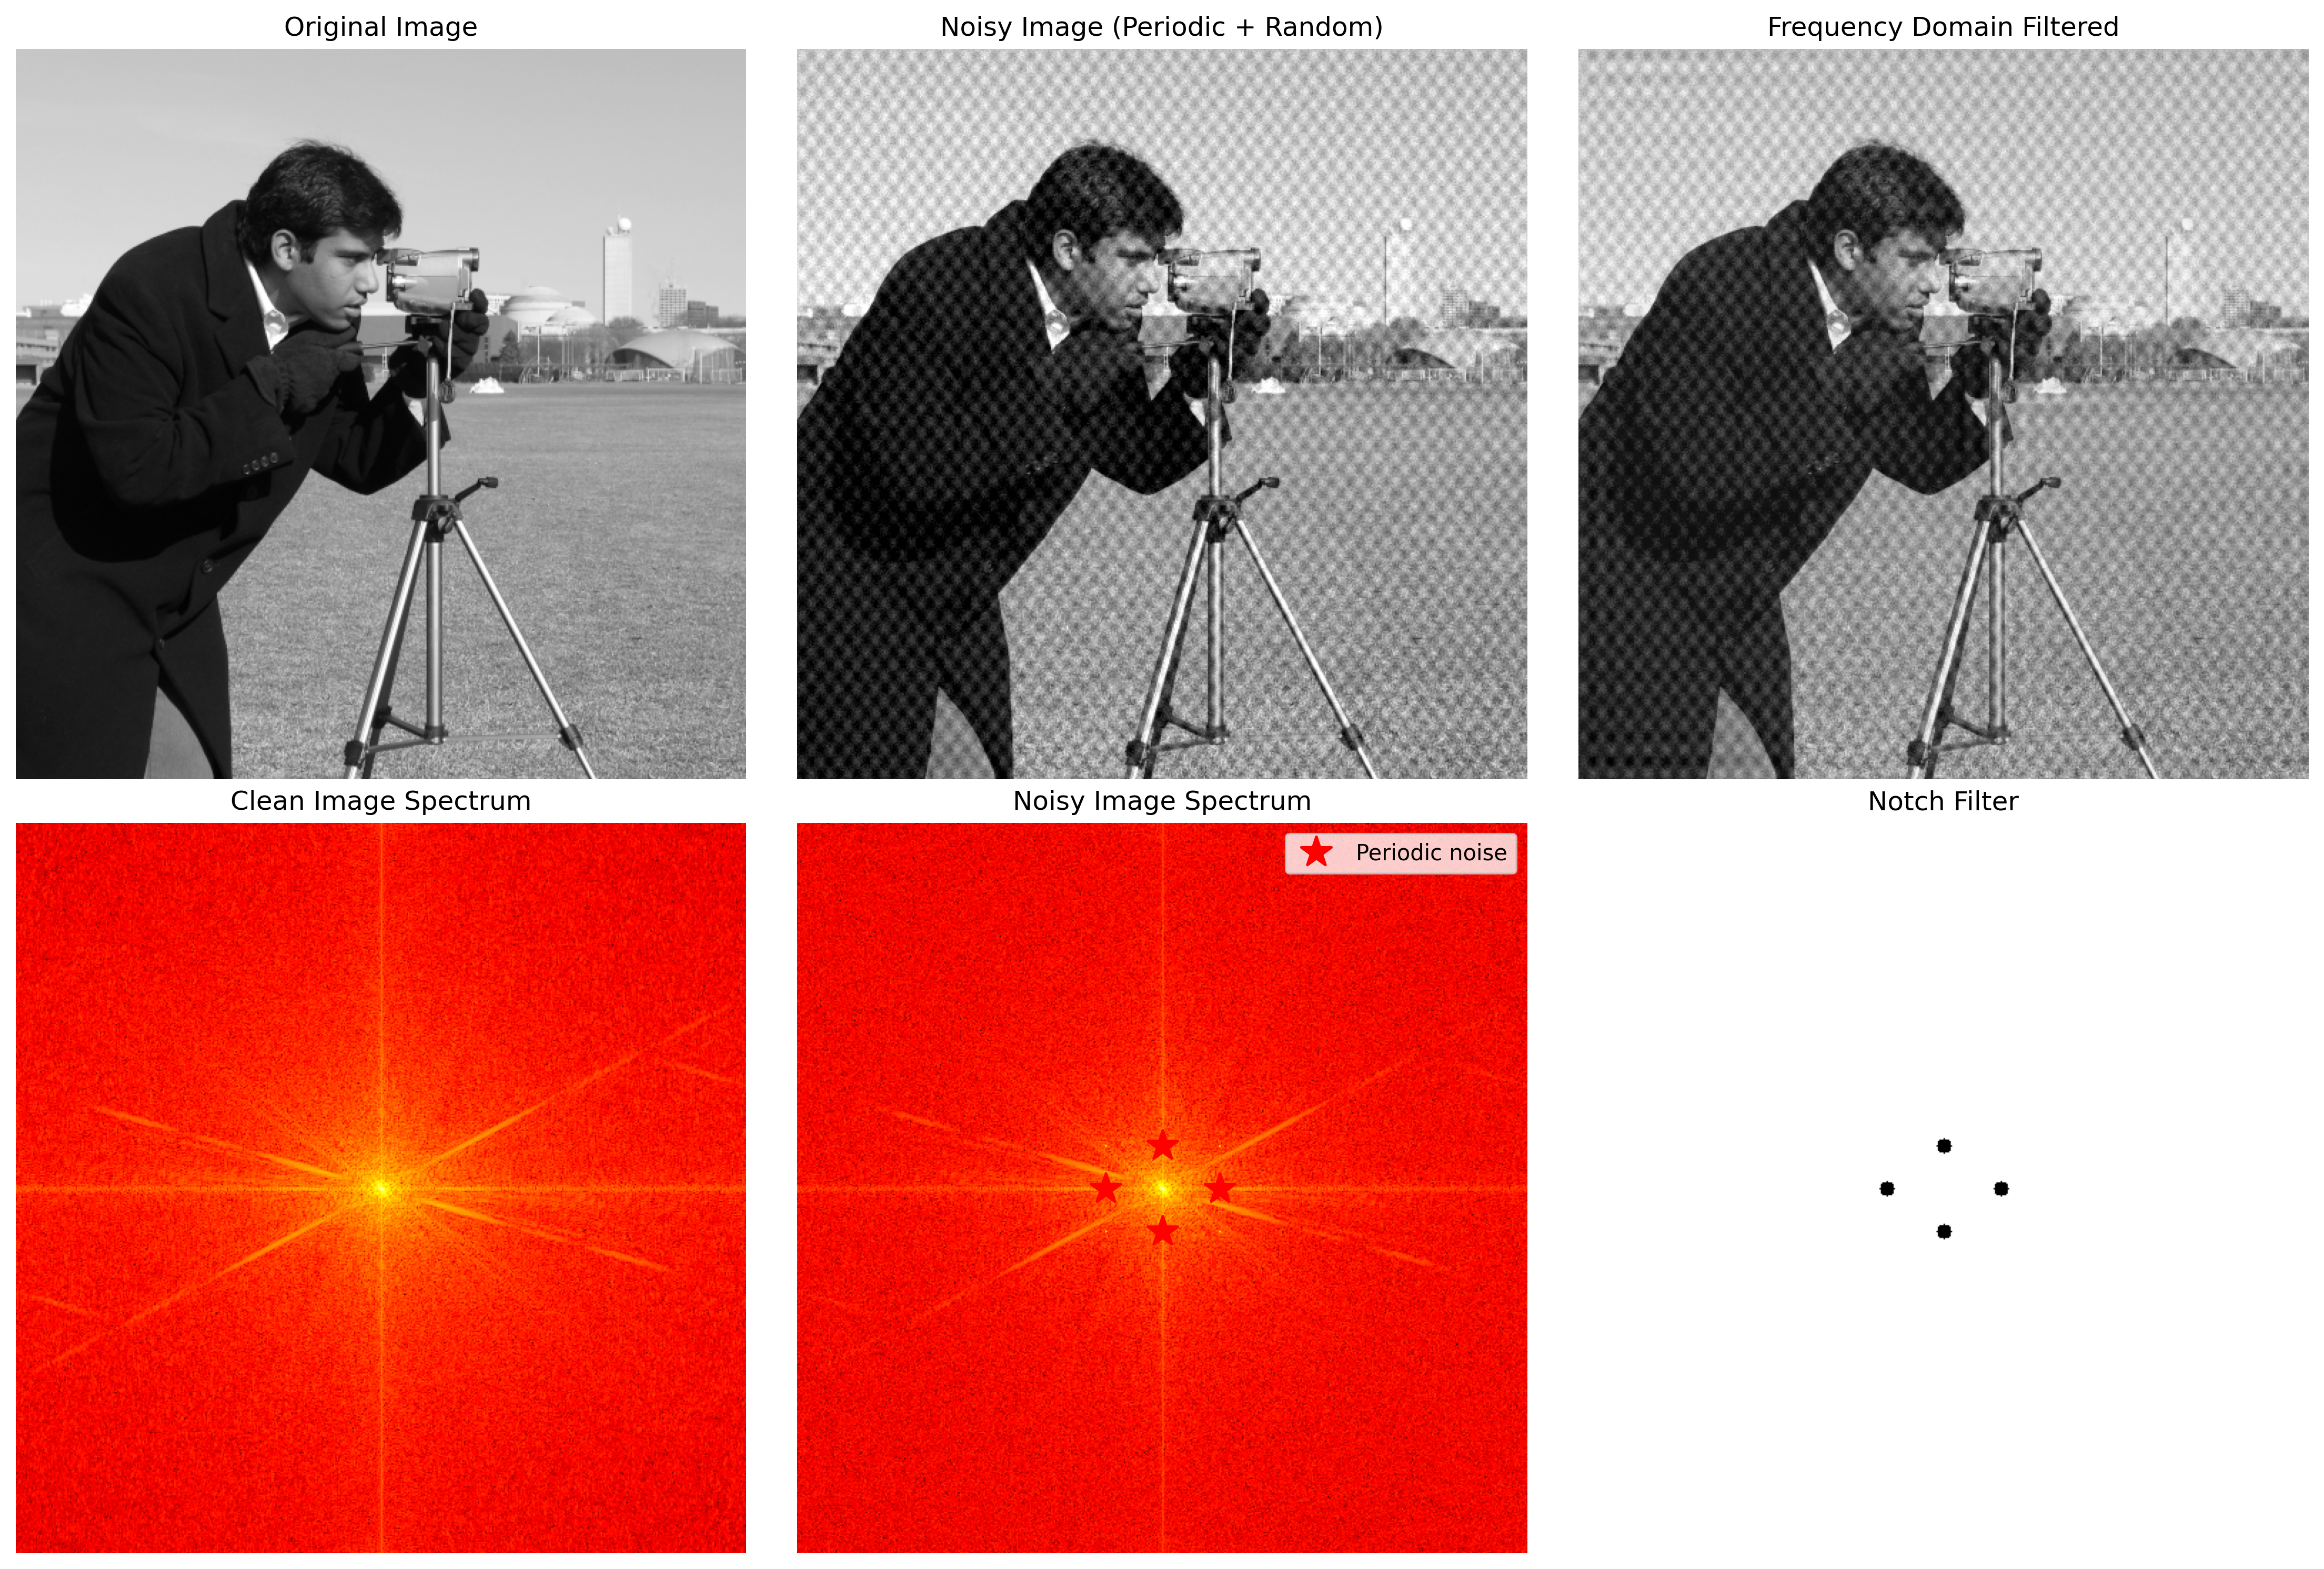
\includegraphics[width=\textwidth]{../figures/frequency_domain_motivation.png}\\
\centering{\small Spatial vs frequency domain representation}
\end{columns}
\end{frame}

\section{Core Theory}

\begin{frame}{2D Fourier Transform}
\begin{columns}
\begin{column}{0.55\textwidth}
\begin{alertblock}{Continuous 2D Fourier Transform}
Forward Transform:
$$F(u,v) = \int_{-\infty}^{\infty} \int_{-\infty}^{\infty} f(x,y) e^{-j2\pi(ux+vy)} dx dy$$

Inverse Transform:
$$f(x,y) = \int_{-\infty}^{\infty} \int_{-\infty}^{\infty} F(u,v) e^{j2\pi(ux+vy)} du dv$$
\end{alertblock}

\textbf{Discrete 2D Fourier Transform (DFT):}
$$F(u,v) = \frac{1}{MN} \sum_{x=0}^{M-1} \sum_{y=0}^{N-1} f(x,y) e^{-j2\pi(ux/M + vy/N)}$$

Where $u = 0,1,\ldots,M-1$ and $v = 0,1,\ldots,N-1$
\end{column}
\begin{column}{0.4\textwidth}
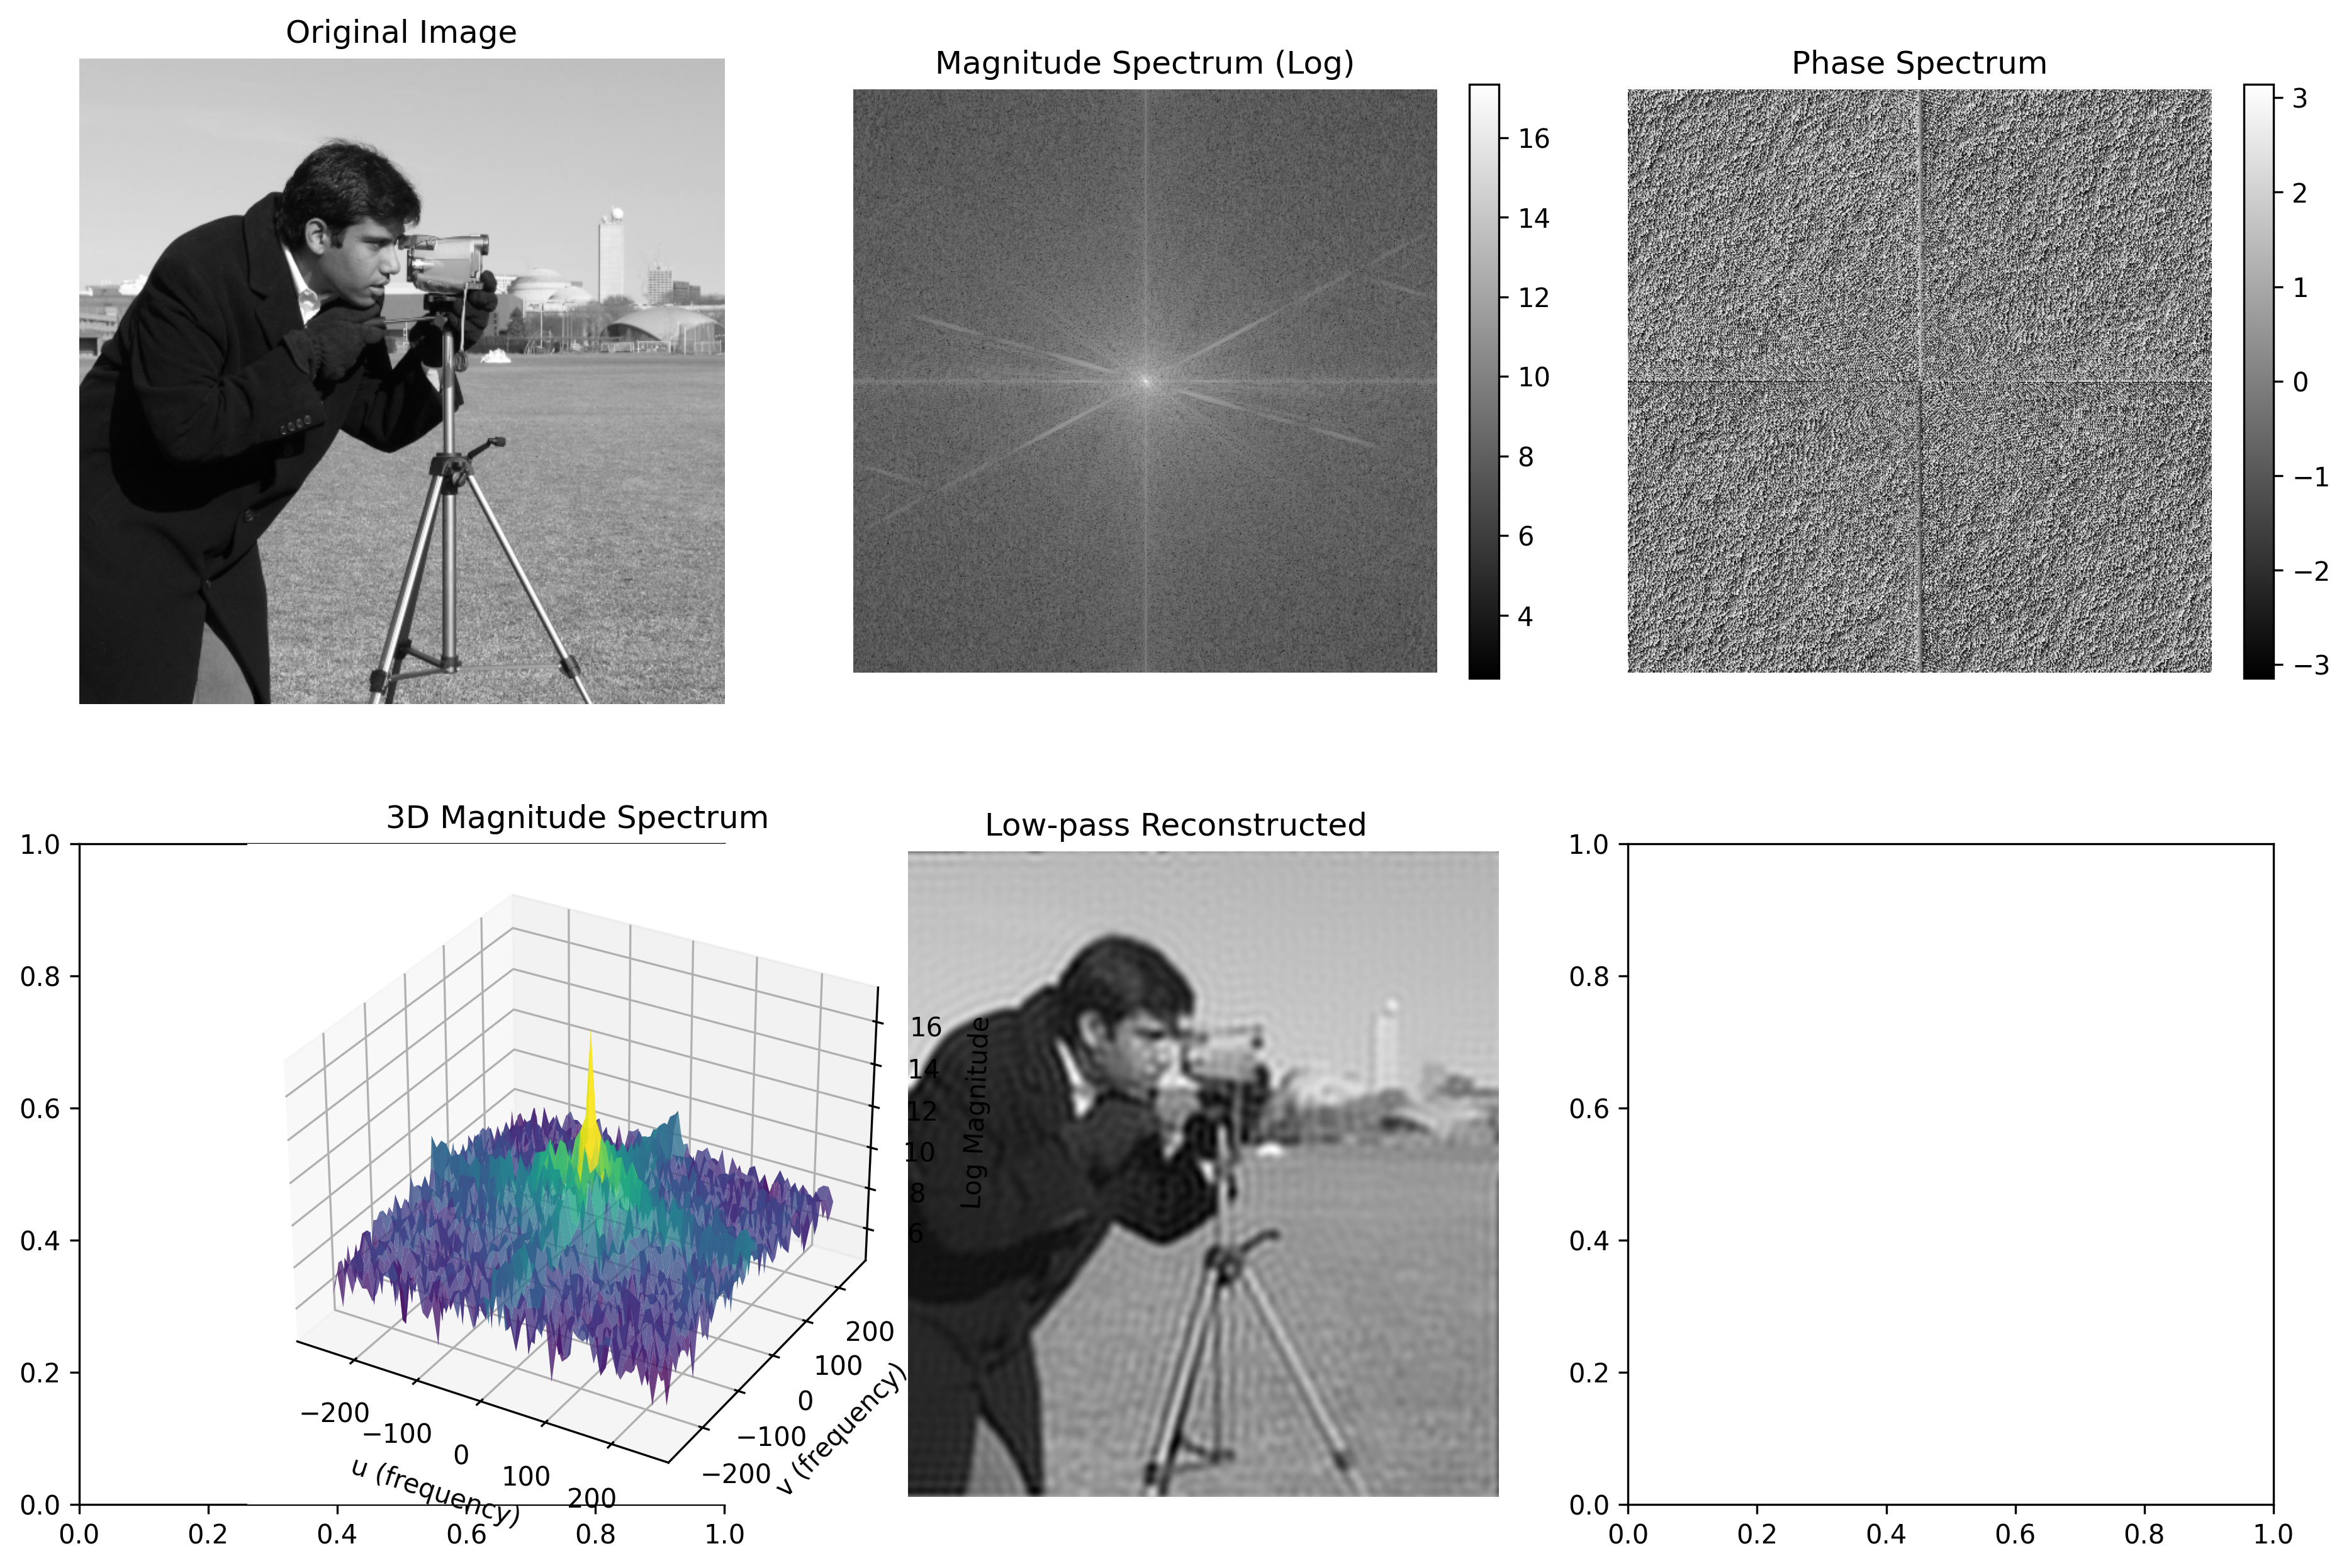
\includegraphics[width=\textwidth]{../figures/fourier_transform_2d.png}\\
\centering{\small 2D Fourier transform visualization}
\end{column}
\end{columns}
\end{frame}

\begin{frame}{Frequency Representation}
\begin{columns}
\begin{column}{0.5\textwidth}
\textbf{Magnitude and Phase:}
$$|F(u,v)| = \sqrt{R^2(u,v) + I^2(u,v)}$$
$$\phi(u,v) = \arctan\left(\frac{I(u,v)}{R(u,v)}\right)$$

Where $R(u,v)$ and $I(u,v)$ are real and imaginary parts.

\textbf{Power Spectrum:}
$$P(u,v) = |F(u,v)|^2$$

\textbf{Frequency Domain Properties:}
\begin{itemize}
\item Low frequencies → smooth variations
\item High frequencies → edges and details
\item Phase → spatial information
\item Magnitude → frequency content strength
\end{itemize}
\end{column}
\begin{column}{0.45\textwidth}
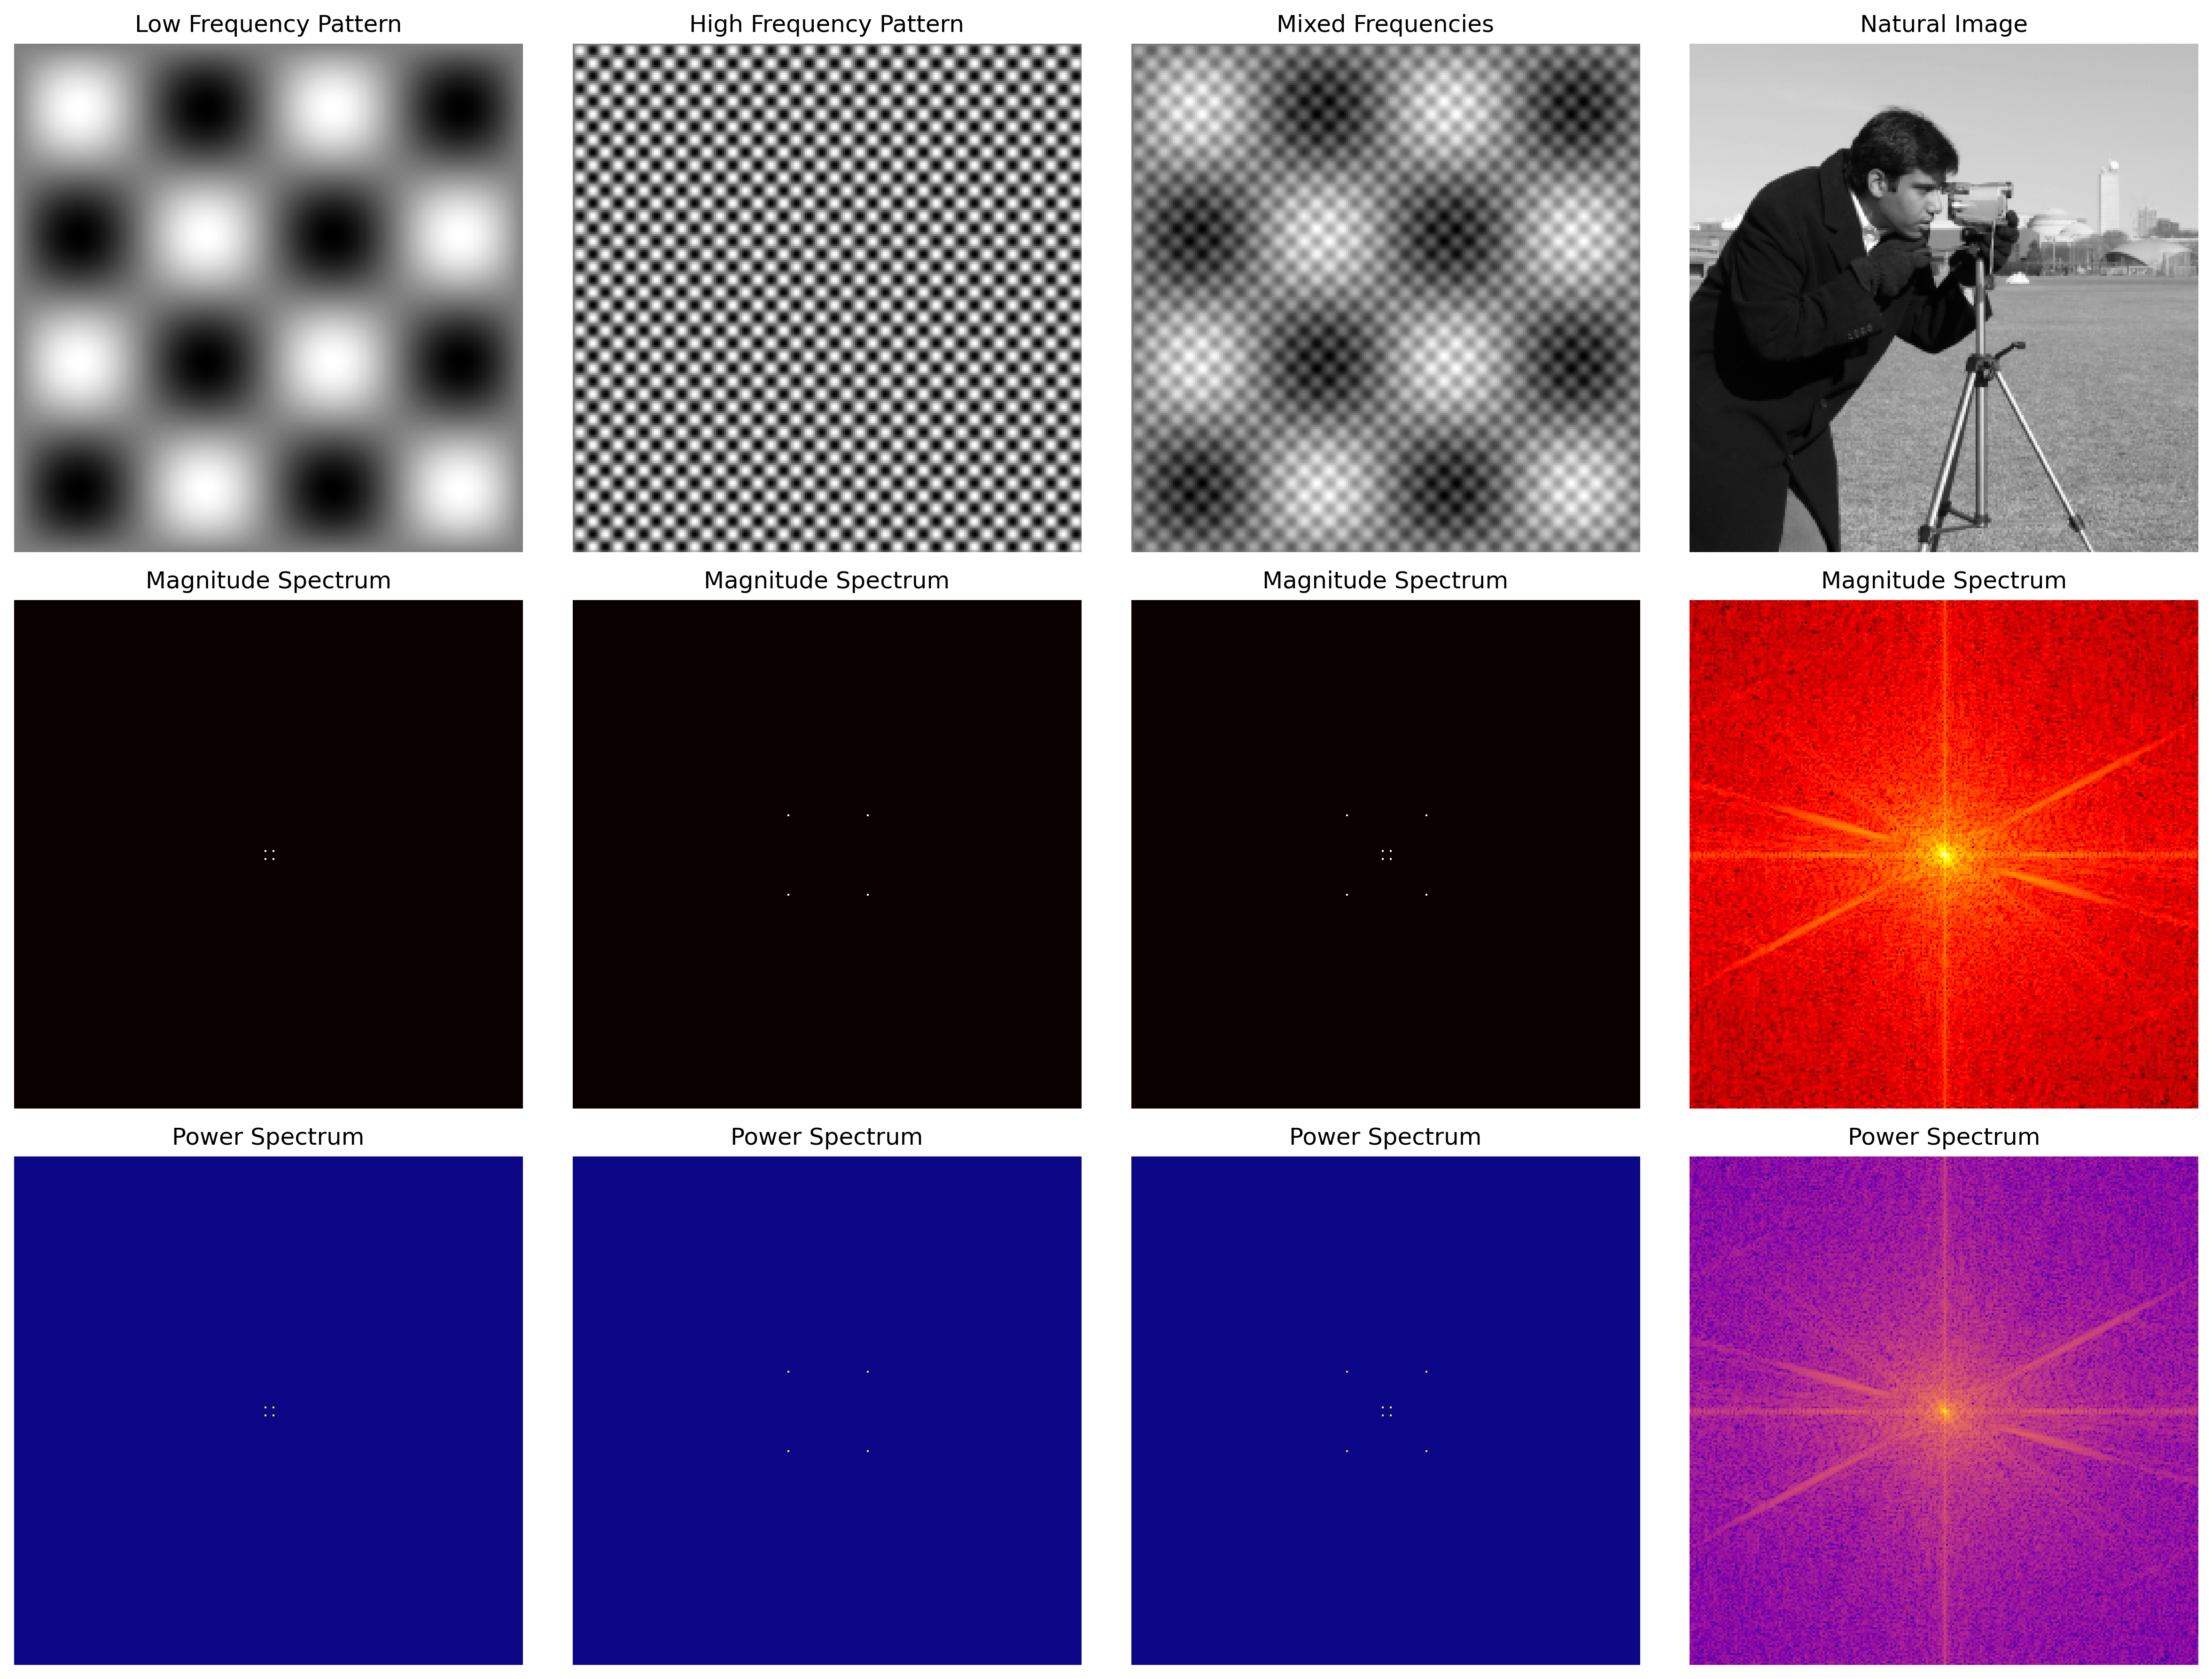
\includegraphics[width=\textwidth]{../figures/frequency_representation.png}\\
\centering{\small Magnitude and phase spectra}
\end{column}
\end{columns}
\end{frame}

\begin{frame}{Frequency Domain Characteristics}
\textbf{Frequency Quadrants:}

\begin{columns}
\column{0.5\textwidth}
\begin{itemize}
\item \textbf{DC Component:} $F(0,0)$ = average intensity
\item \textbf{Low frequencies:} Near origin, smooth variations
\item \textbf{High frequencies:} Away from origin, fine details
\item \textbf{Symmetry:} $F(u,v) = F^*(-u,-v)$ for real images
\end{itemize}

\textbf{Frequency Interpretation:}
\begin{align}
u &= \text{horizontal frequency} \\
v &= \text{vertical frequency} \\
\sqrt{u^2 + v^2} &= \text{radial frequency}
\end{align}

\column{0.45\textwidth}
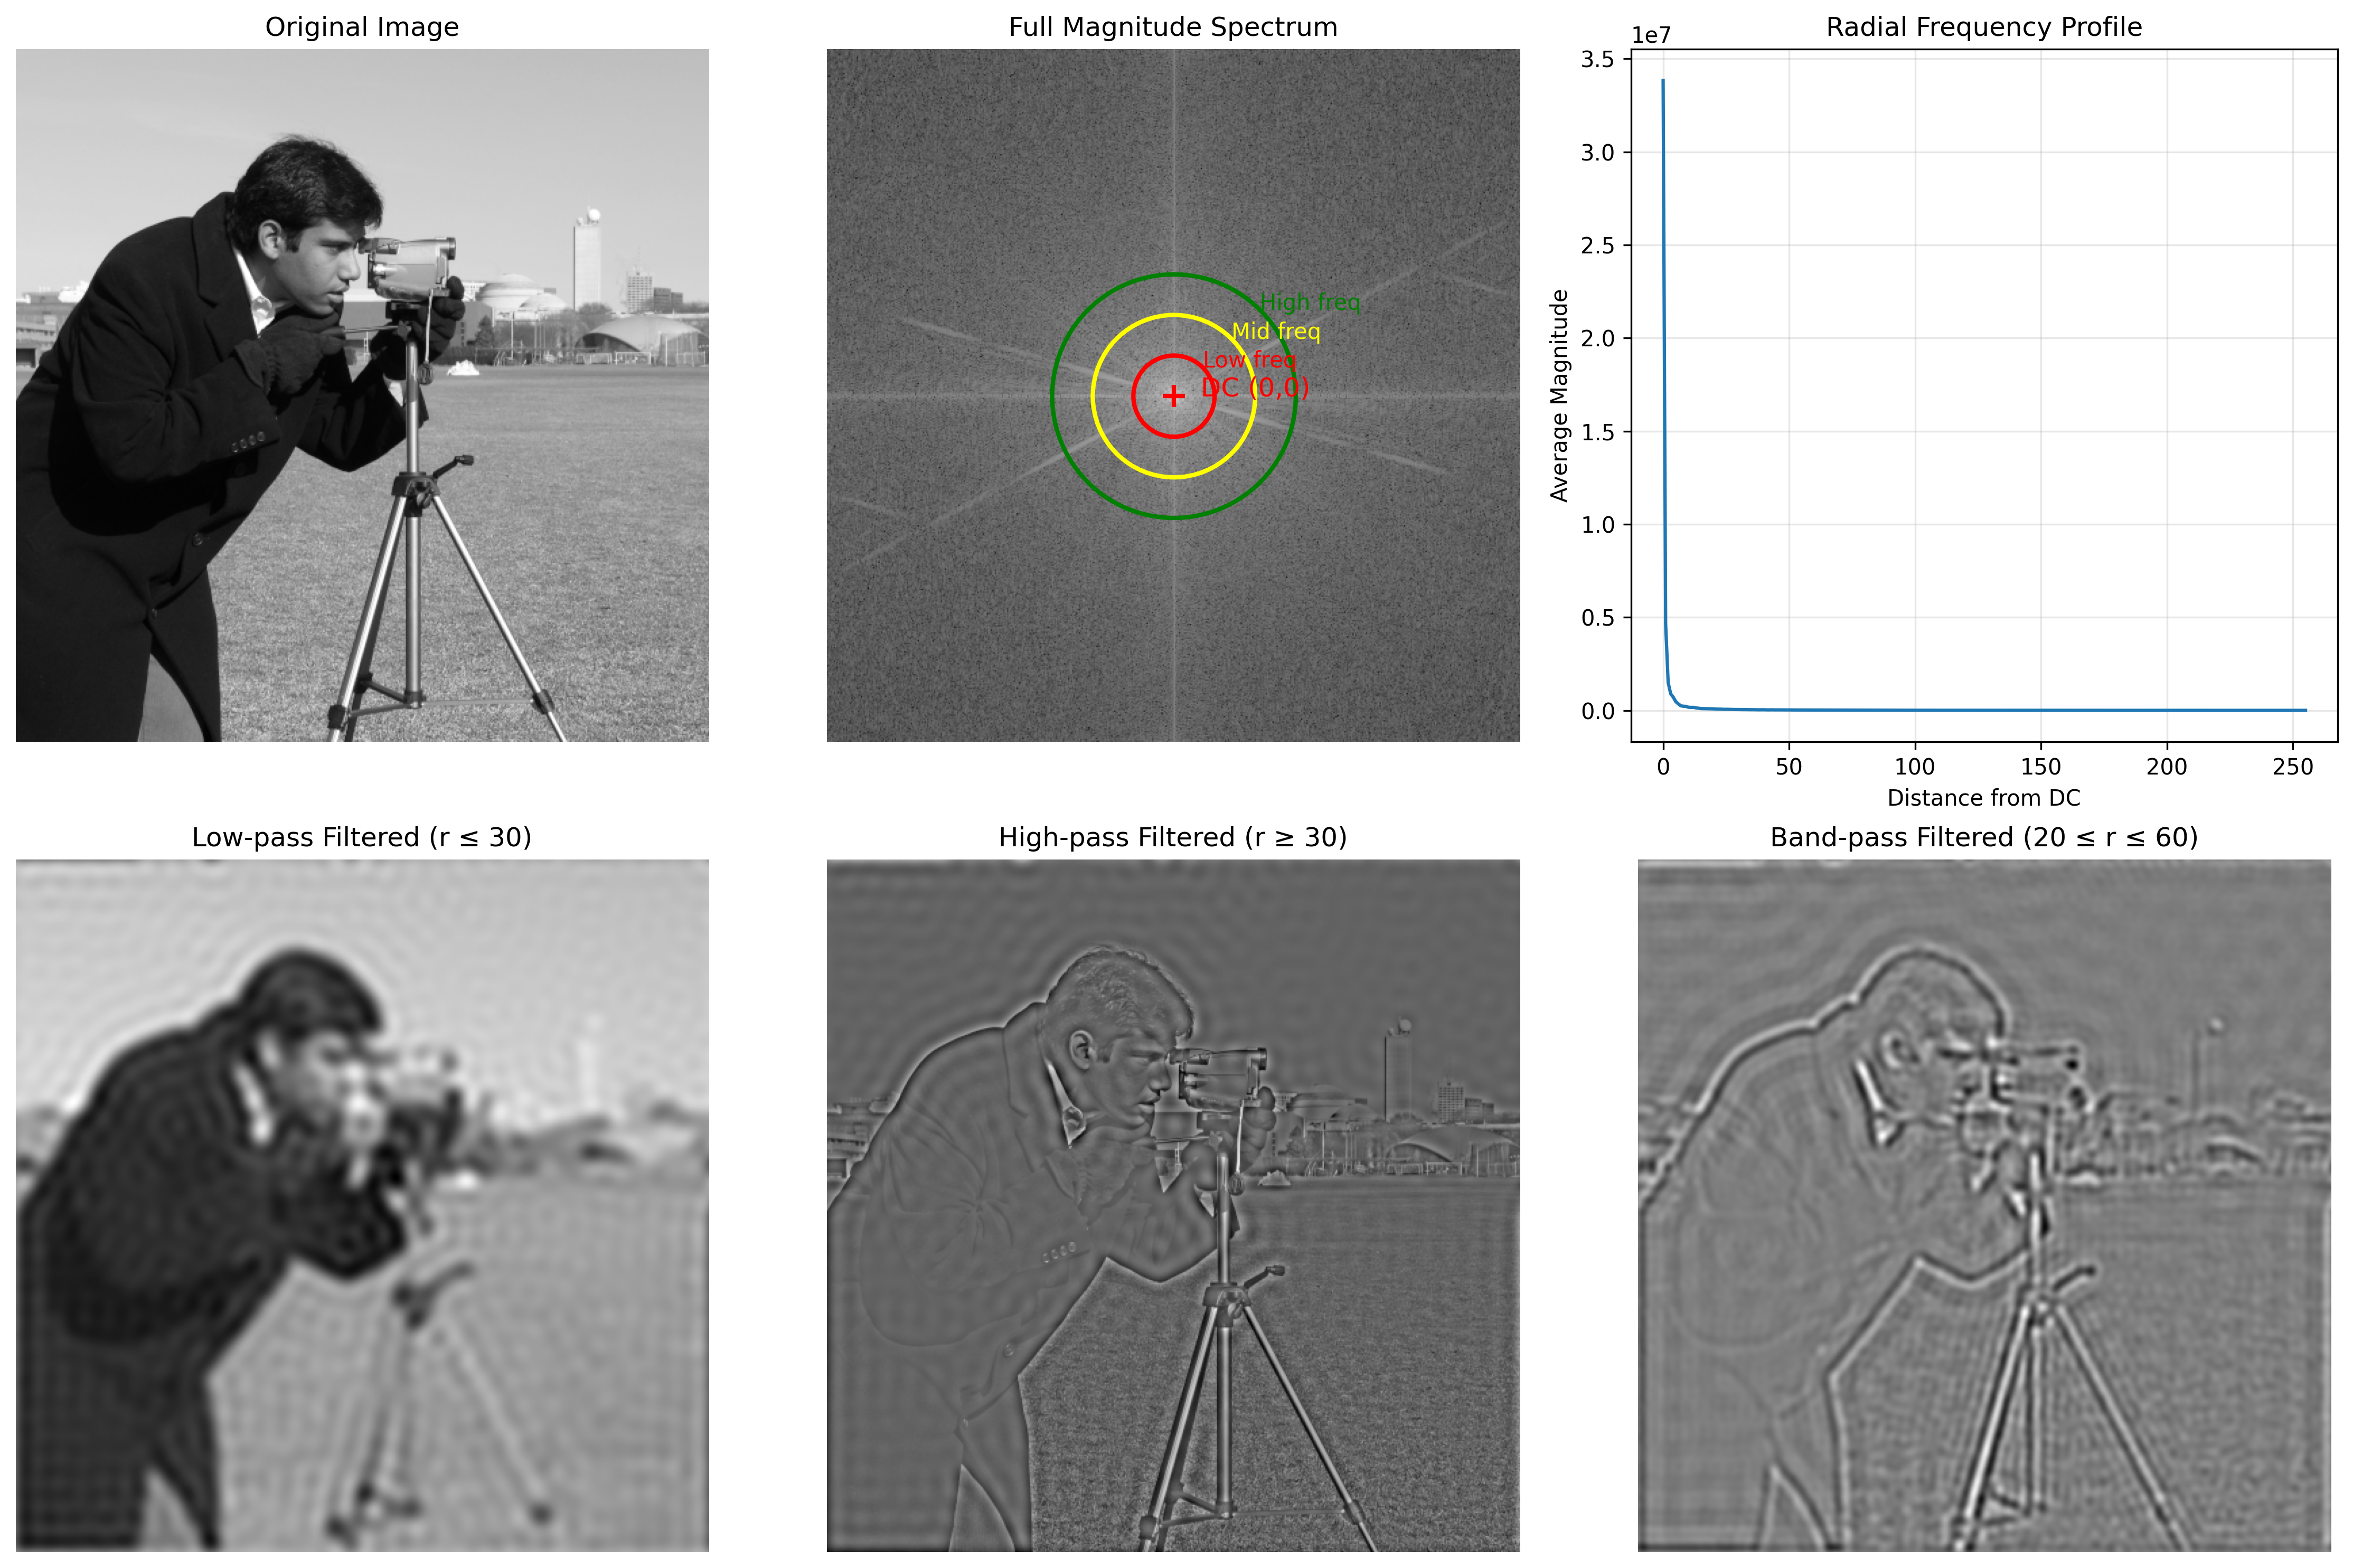
\includegraphics[width=\textwidth]{../figures/frequency_quadrants.png}\\
\centering{\small Frequency domain quadrants and interpretation}
\end{columns}
\end{frame}

\section{Methods and Algorithms}

\begin{frame}{Low-Pass Filtering}
\begin{columns}
\begin{column}{0.55\textwidth}
\textbf{Purpose:} Remove high-frequency components (noise, fine details)

\textbf{Ideal Low-Pass Filter:}
$$H(u,v) = \begin{cases}
1 & \text{if } D(u,v) \leq D_0 \\
0 & \text{if } D(u,v) > D_0
\end{cases}$$

Where $D(u,v) = \sqrt{(u-M/2)^2 + (v-N/2)^2}$

\textbf{Butterworth Low-Pass Filter:}
$$H(u,v) = \frac{1}{1 + \left[\frac{D(u,v)}{D_0}\right]^{2n}}$$

\textbf{Gaussian Low-Pass Filter:}
$$H(u,v) = e^{-\frac{D^2(u,v)}{2D_0^2}}$$
\end{column}
\begin{column}{0.4\textwidth}
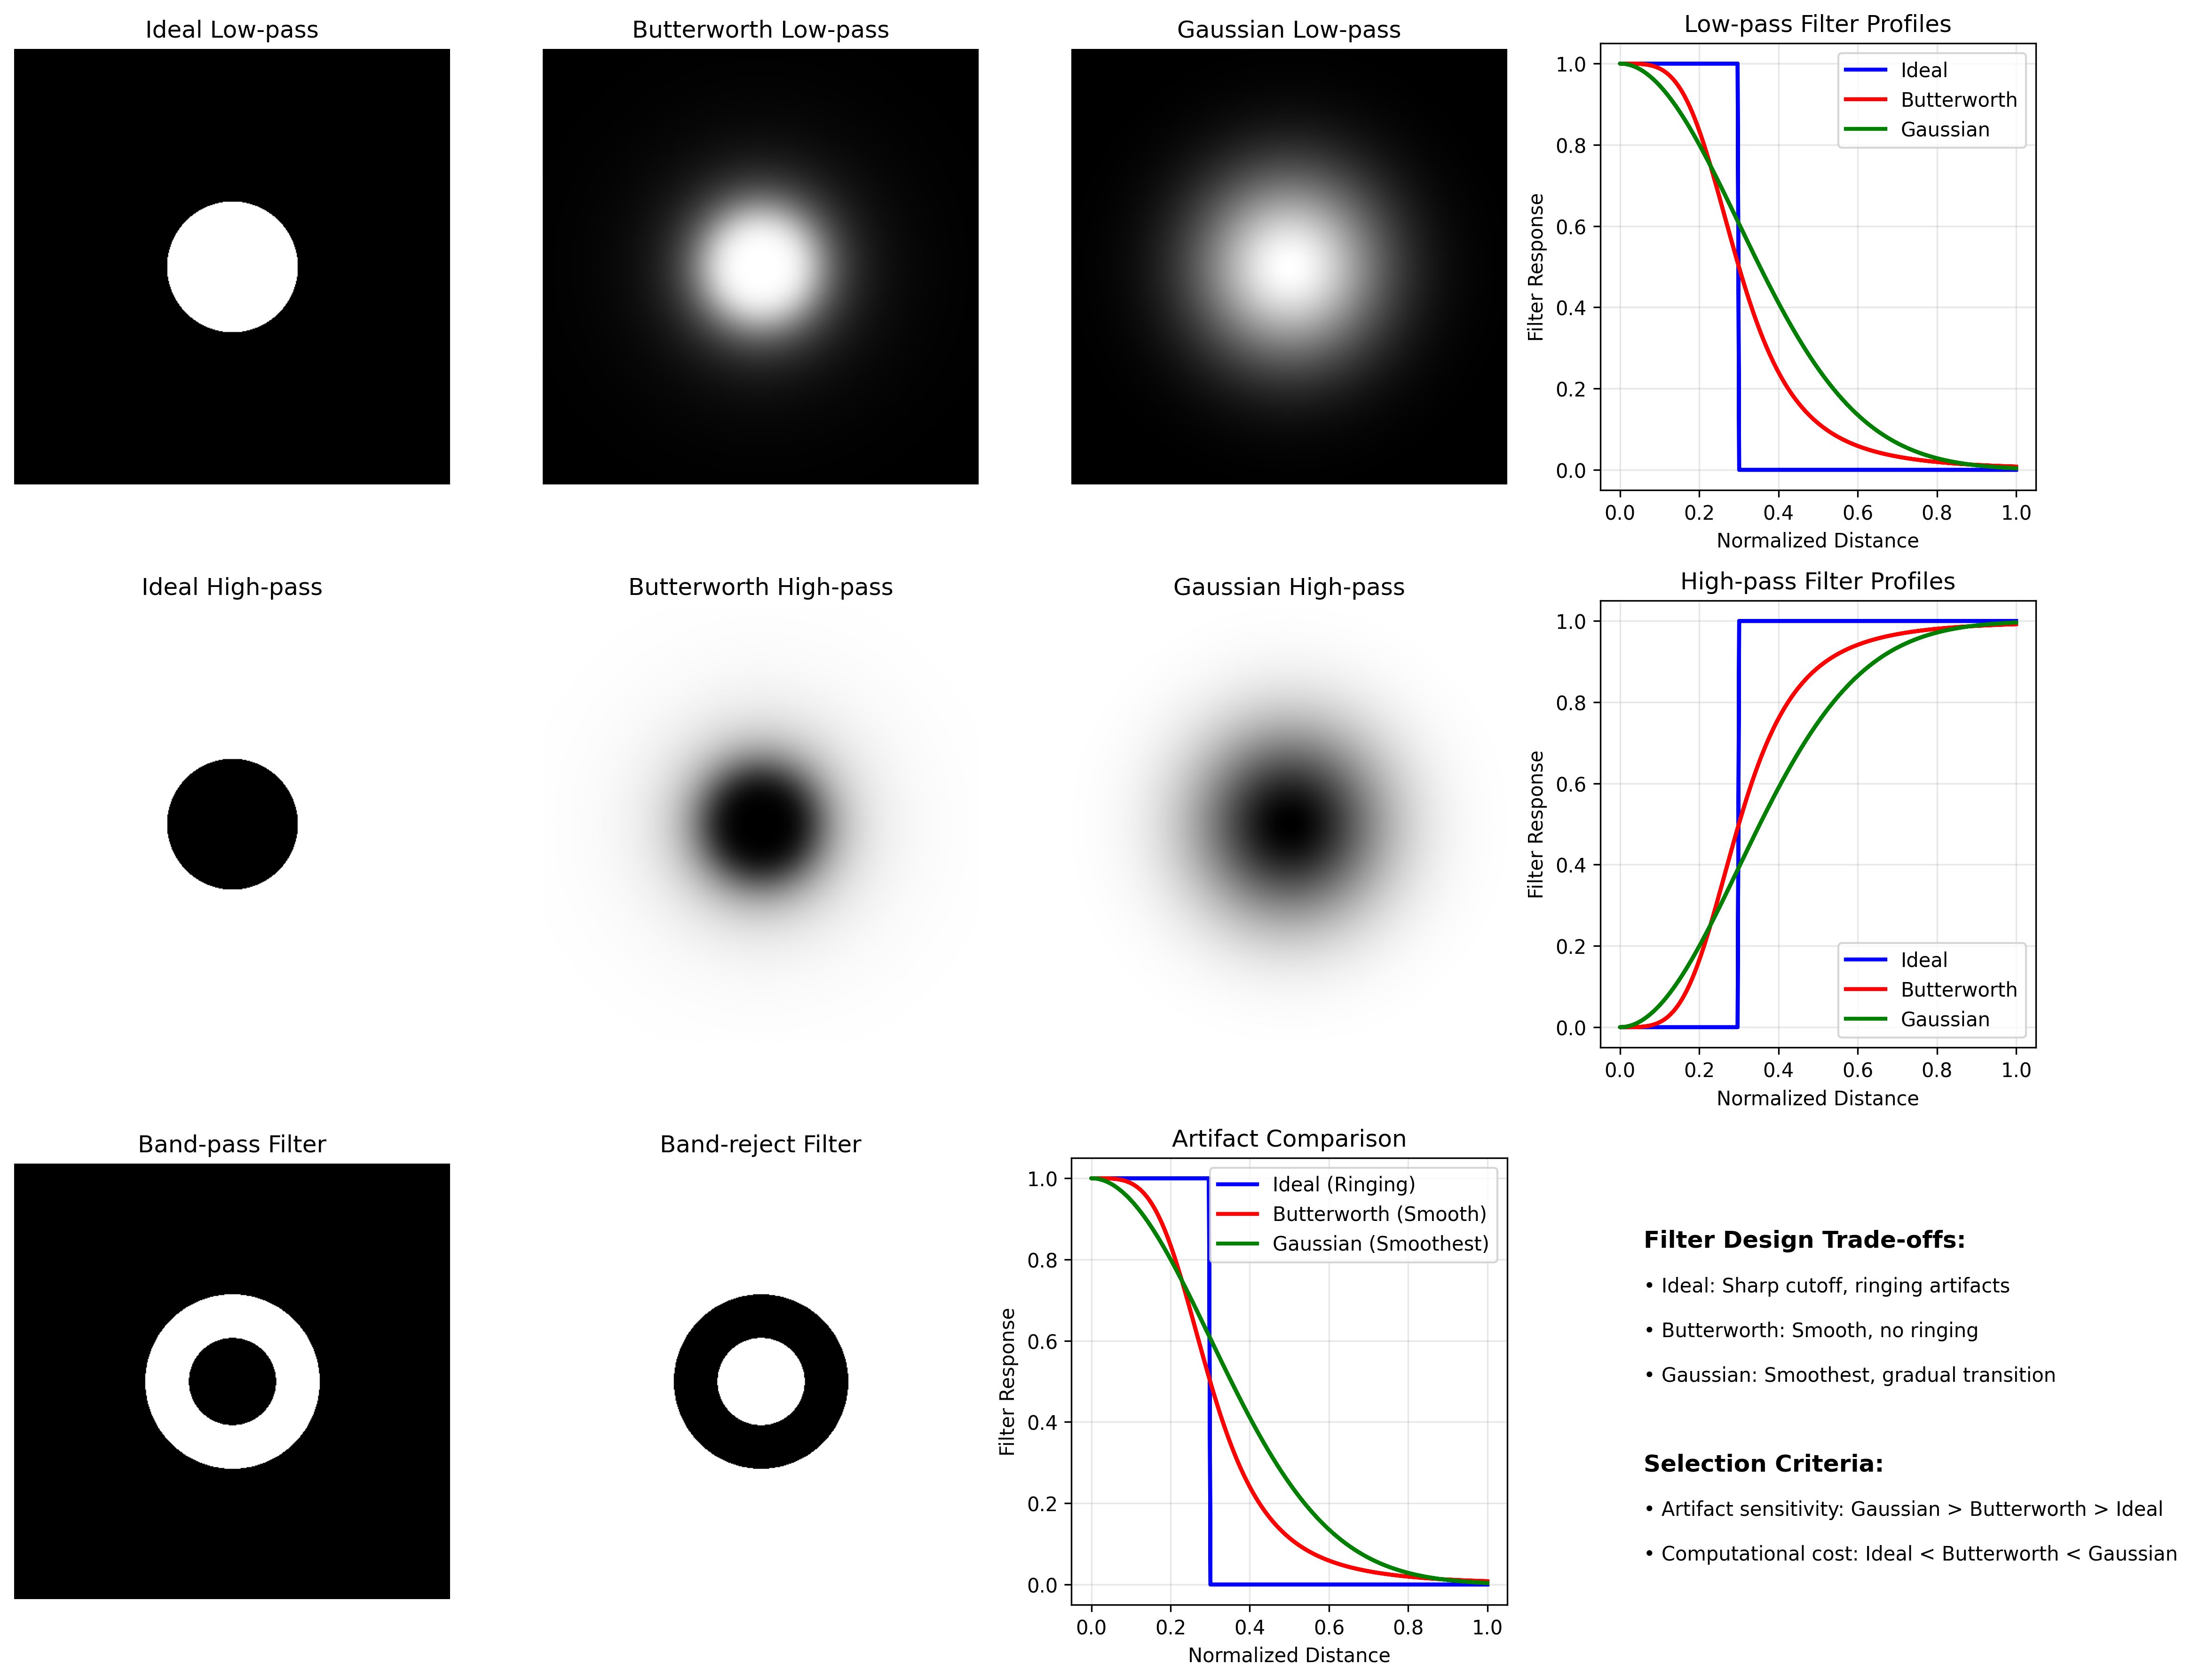
\includegraphics[width=\textwidth]{../figures/low_pass_filters.png}\\
\centering{\small Low-pass filter profiles and effects}
\end{column}
\end{columns}
\end{frame}

\begin{frame}{High-Pass Filtering}
\begin{columns}
\begin{column}{0.55\textwidth}
\textbf{Purpose:} Enhance edges and fine details, remove smooth variations

\textbf{Ideal High-Pass Filter:}
$$H(u,v) = \begin{cases}
0 & \text{if } D(u,v) \leq D_0 \\
1 & \text{if } D(u,v) > D_0
\end{cases}$$

\textbf{Butterworth High-Pass Filter:}
$$H(u,v) = \frac{1}{1 + \left[\frac{D_0}{D(u,v)}\right]^{2n}}$$

\textbf{Gaussian High-Pass Filter:}
$$H(u,v) = 1 - e^{-\frac{D^2(u,v)}{2D_0^2}}$$

\textbf{High-Frequency Emphasis:}
$$H_{hfe}(u,v) = a + b \cdot H_{hp}(u,v)$$
\end{column}
\begin{column}{0.4\textwidth}
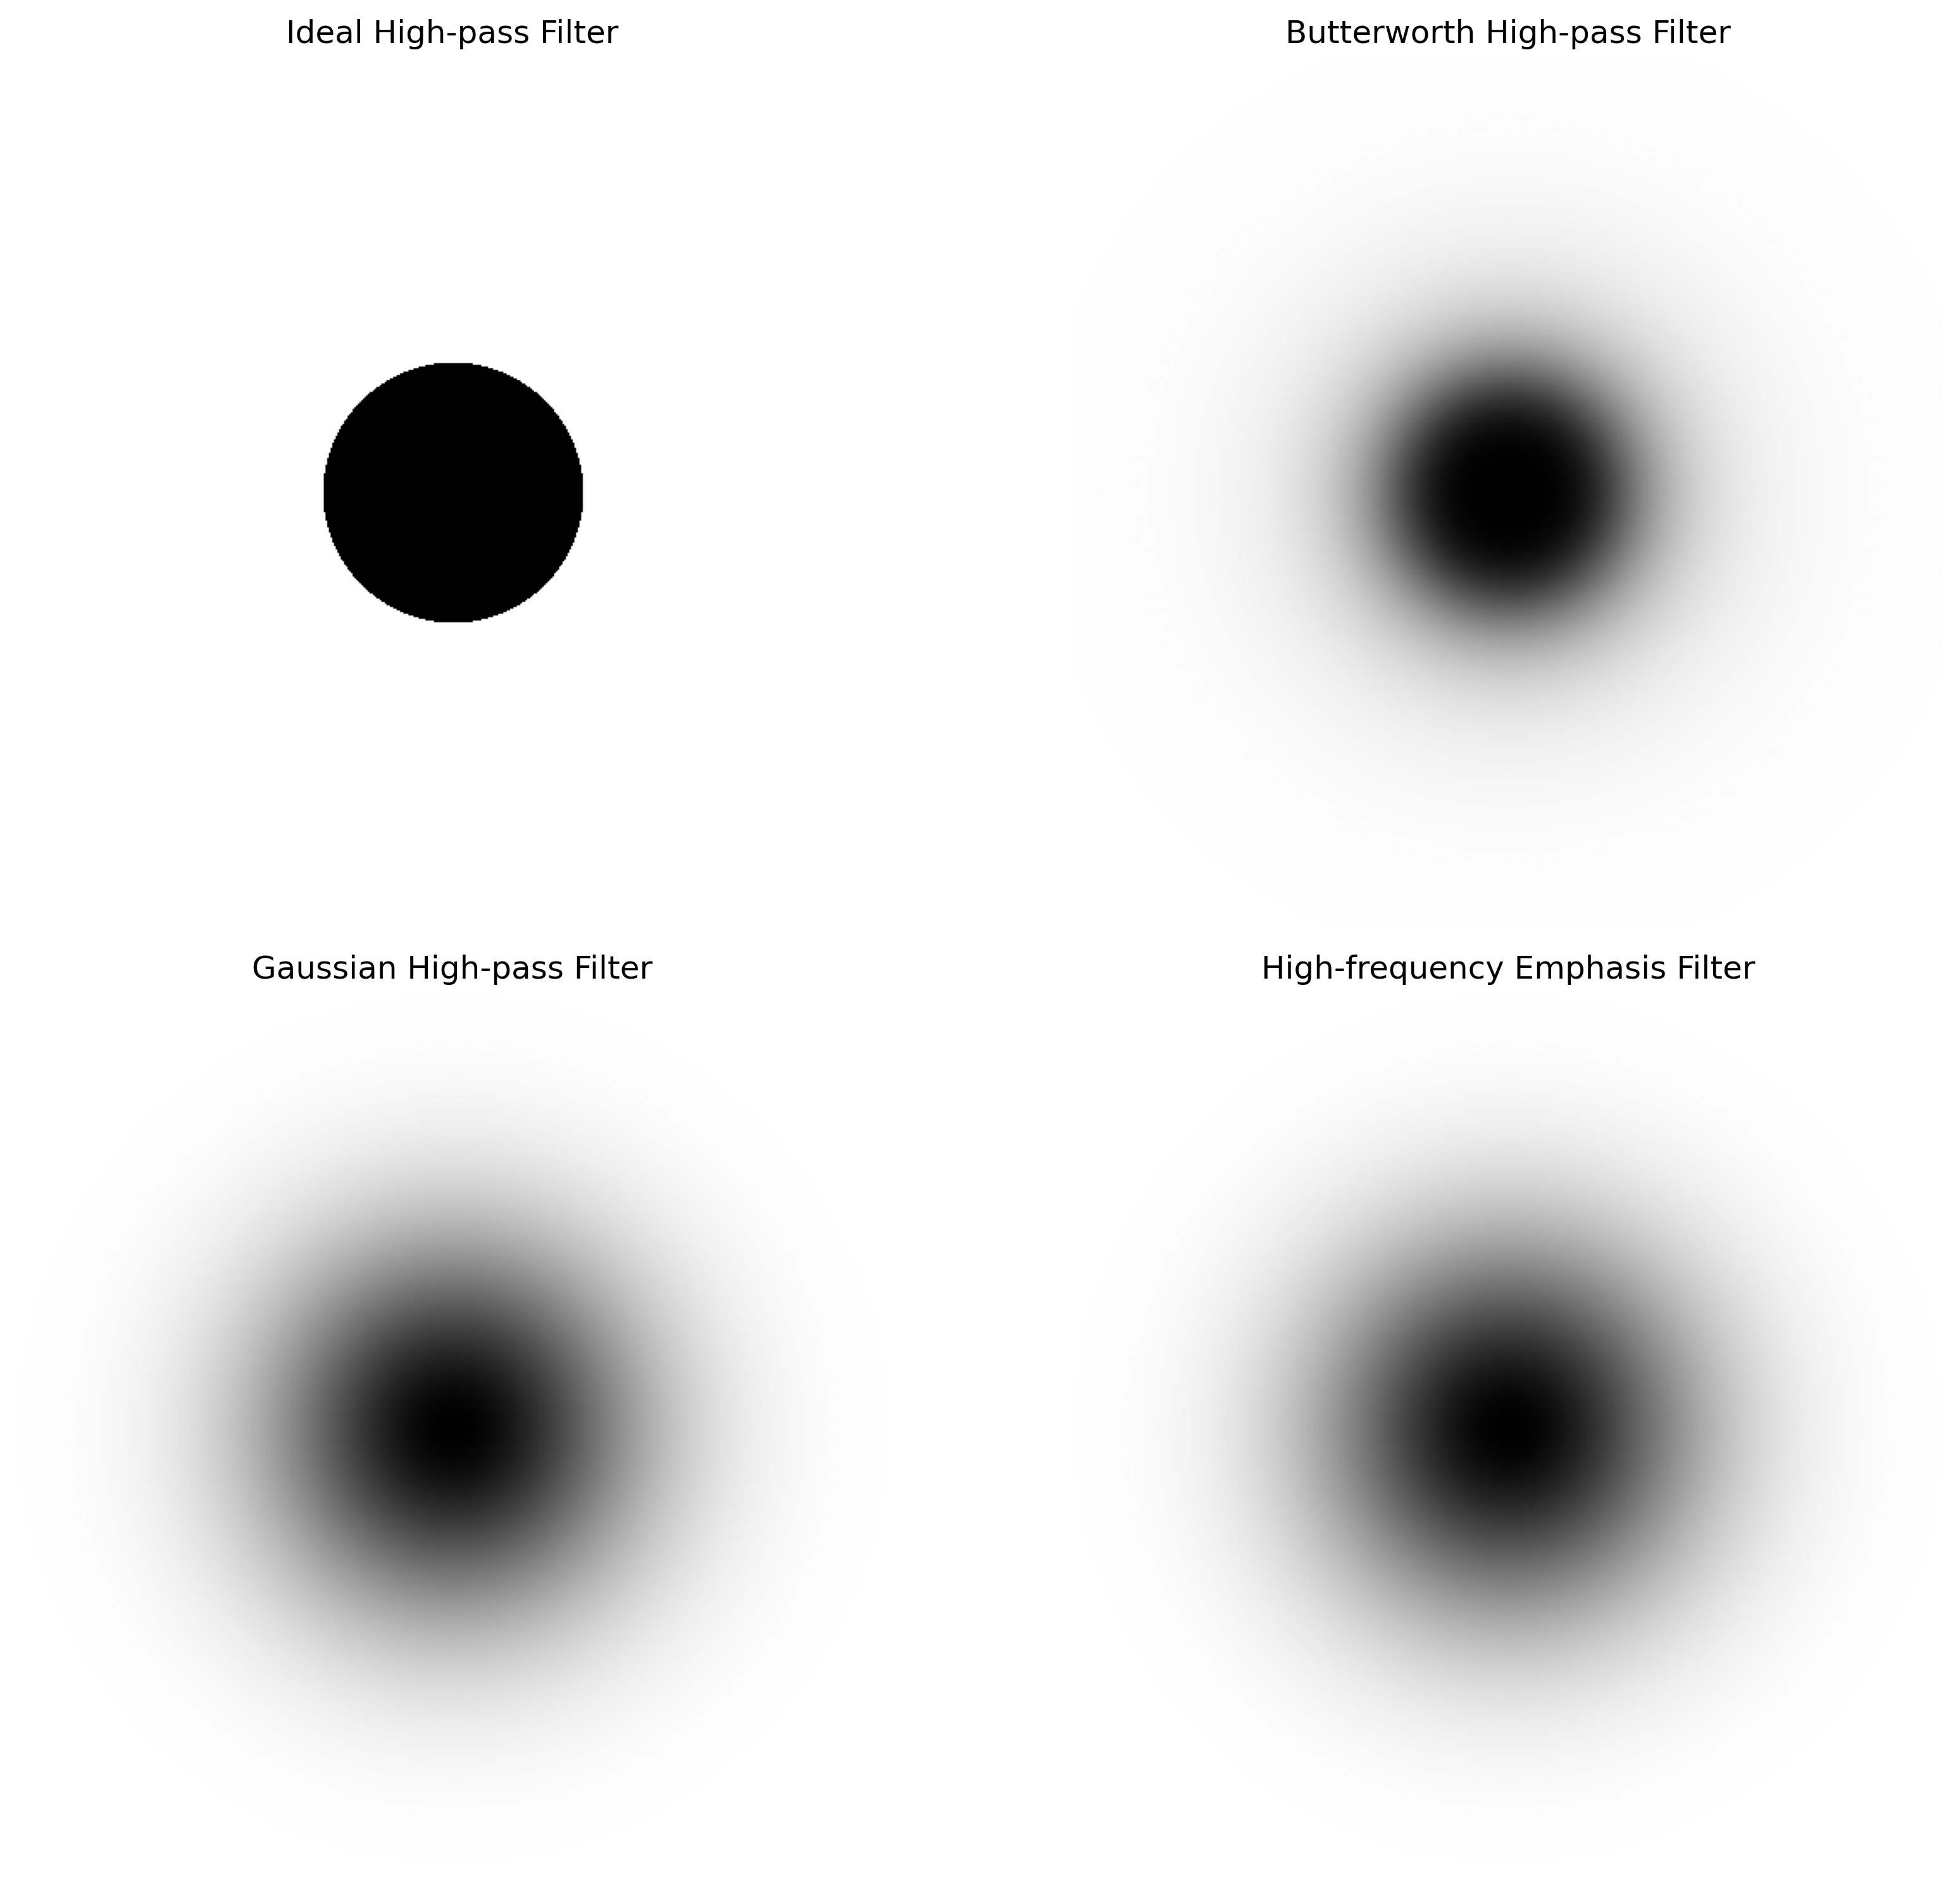
\includegraphics[width=\textwidth]{../figures/high_pass_filters.png}\\
\centering{\small High-pass filter profiles and edge enhancement}
\end{column}
\end{columns}
\end{frame}

\begin{frame}{Band-Pass Filtering}
\begin{columns}
\begin{column}{0.55\textwidth}
\textbf{Purpose:} Pass specific frequency ranges, useful for periodic noise removal

\textbf{Band-Pass Filter:}
$$H_{bp}(u,v) = H_{hp1}(u,v) \cdot H_{lp2}(u,v)$$

Where $H_{hp1}$ has cutoff $D_1$ and $H_{lp2}$ has cutoff $D_2 > D_1$

\textbf{Band-Reject (Notch) Filter:}
$$H_{br}(u,v) = 1 - H_{bp}(u,v)$$

\textbf{Selective Frequency Filtering:}
\begin{align}
H_{notch}(u,v) &= \prod_{k} H_k(u,v) \\
H_k(u,v) &= \frac{1}{1 + \left[\frac{D_k \cdot W}{D_k^2(u,v) - D_0^2}\right]^{2n}}
\end{align}

For multiple notch frequencies $D_0^{(k)}$
\end{column}
\begin{column}{0.4\textwidth}
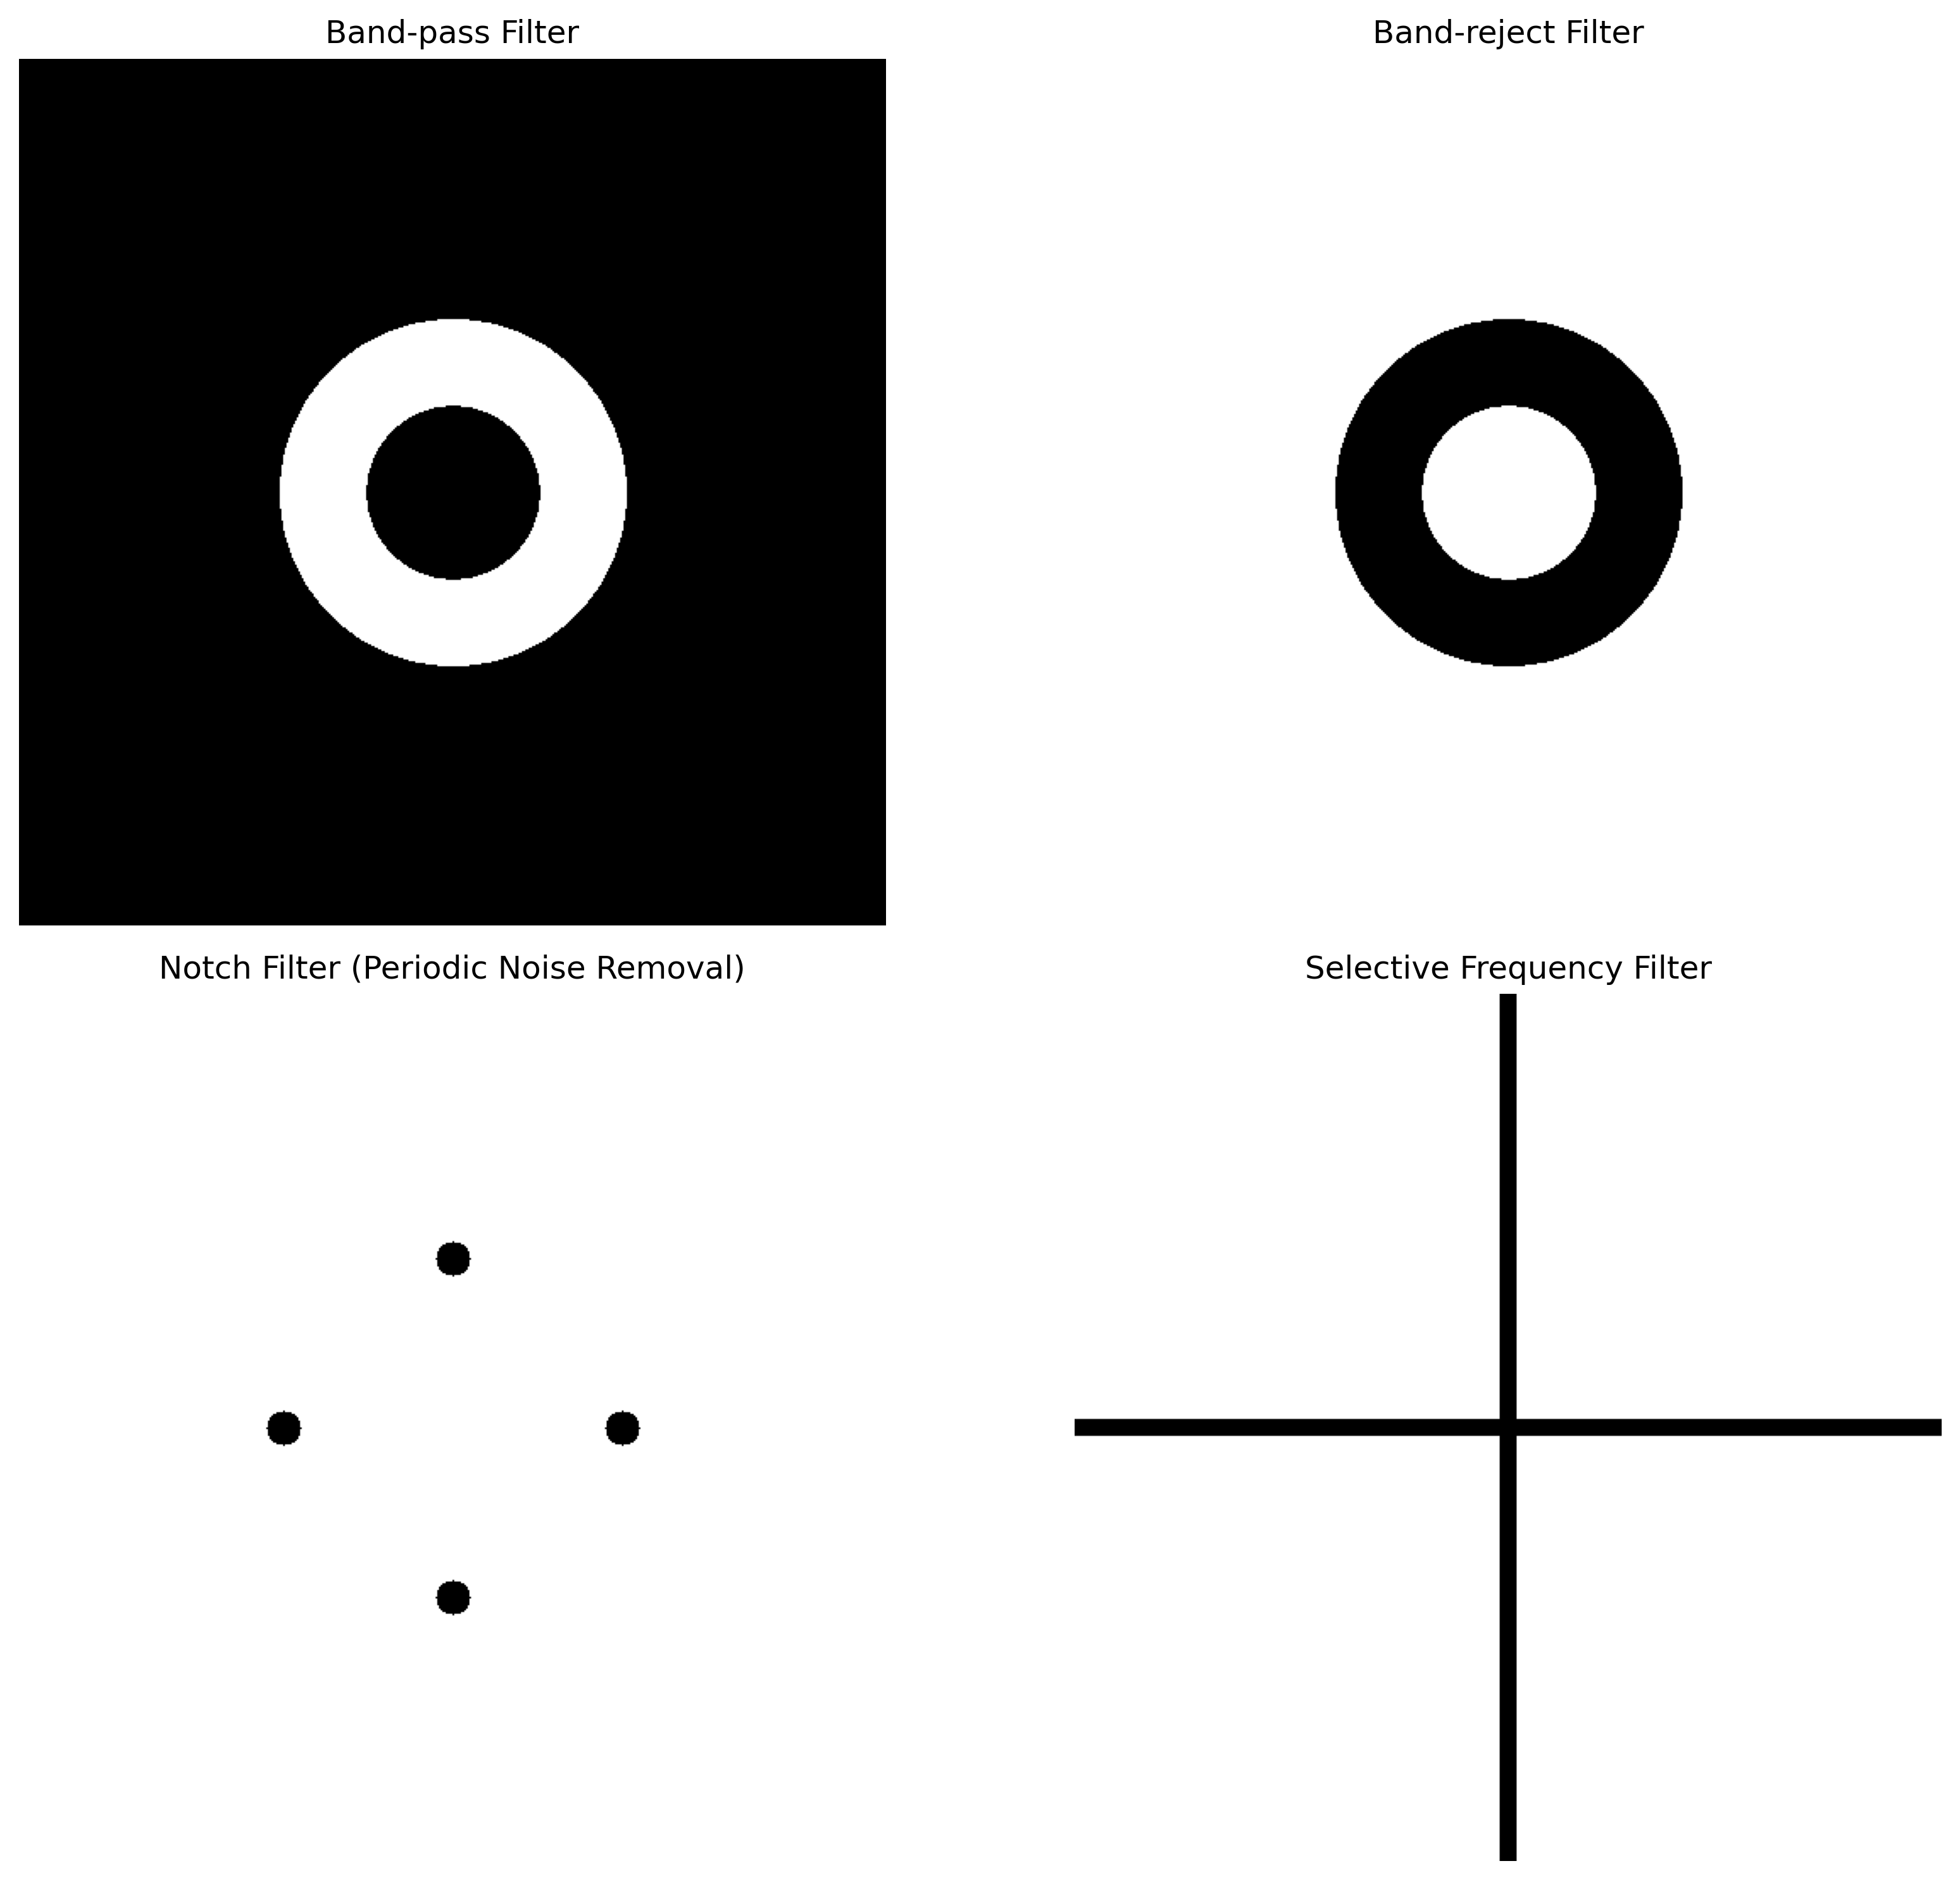
\includegraphics[width=\textwidth]{../figures/band_pass_filters.png}\\
\centering{\small Band-pass and band-reject filter characteristics}
\end{column}
\end{columns}
\end{frame}

\begin{frame}{Fast Fourier Transform (FFT)}
\textbf{Computational Efficiency:}

\begin{columns}
\column{0.6\textwidth}
\textbf{DFT Complexity:} $O(N^4)$ for $N \times N$ image
\textbf{FFT Complexity:} $O(N^2 \log N)$ for $N \times N$ image

\textbf{FFT Requirements:}
\begin{itemize}
\item Image dimensions must be powers of 2
\item Zero-padding for arbitrary sizes
\item Periodic boundary assumptions
\end{itemize}

\textbf{2D FFT Implementation:}
\begin{enumerate}
\item Apply 1D FFT to each row
\item Apply 1D FFT to each column of result
\end{enumerate}

\textbf{Frequency Domain Filtering Steps:}
\begin{enumerate}
\item Preprocess: center spectrum using $(-1)^{x+y}$
\item Compute FFT: $F(u,v) = \text{FFT}\{f(x,y)\}$
\item Apply filter: $G(u,v) = H(u,v) \cdot F(u,v)$
\item Inverse FFT: $g(x,y) = \text{IFFT}\{G(u,v)\}$
\item Postprocess: extract real part, re-center
\end{enumerate}

\column{0.35\textwidth}
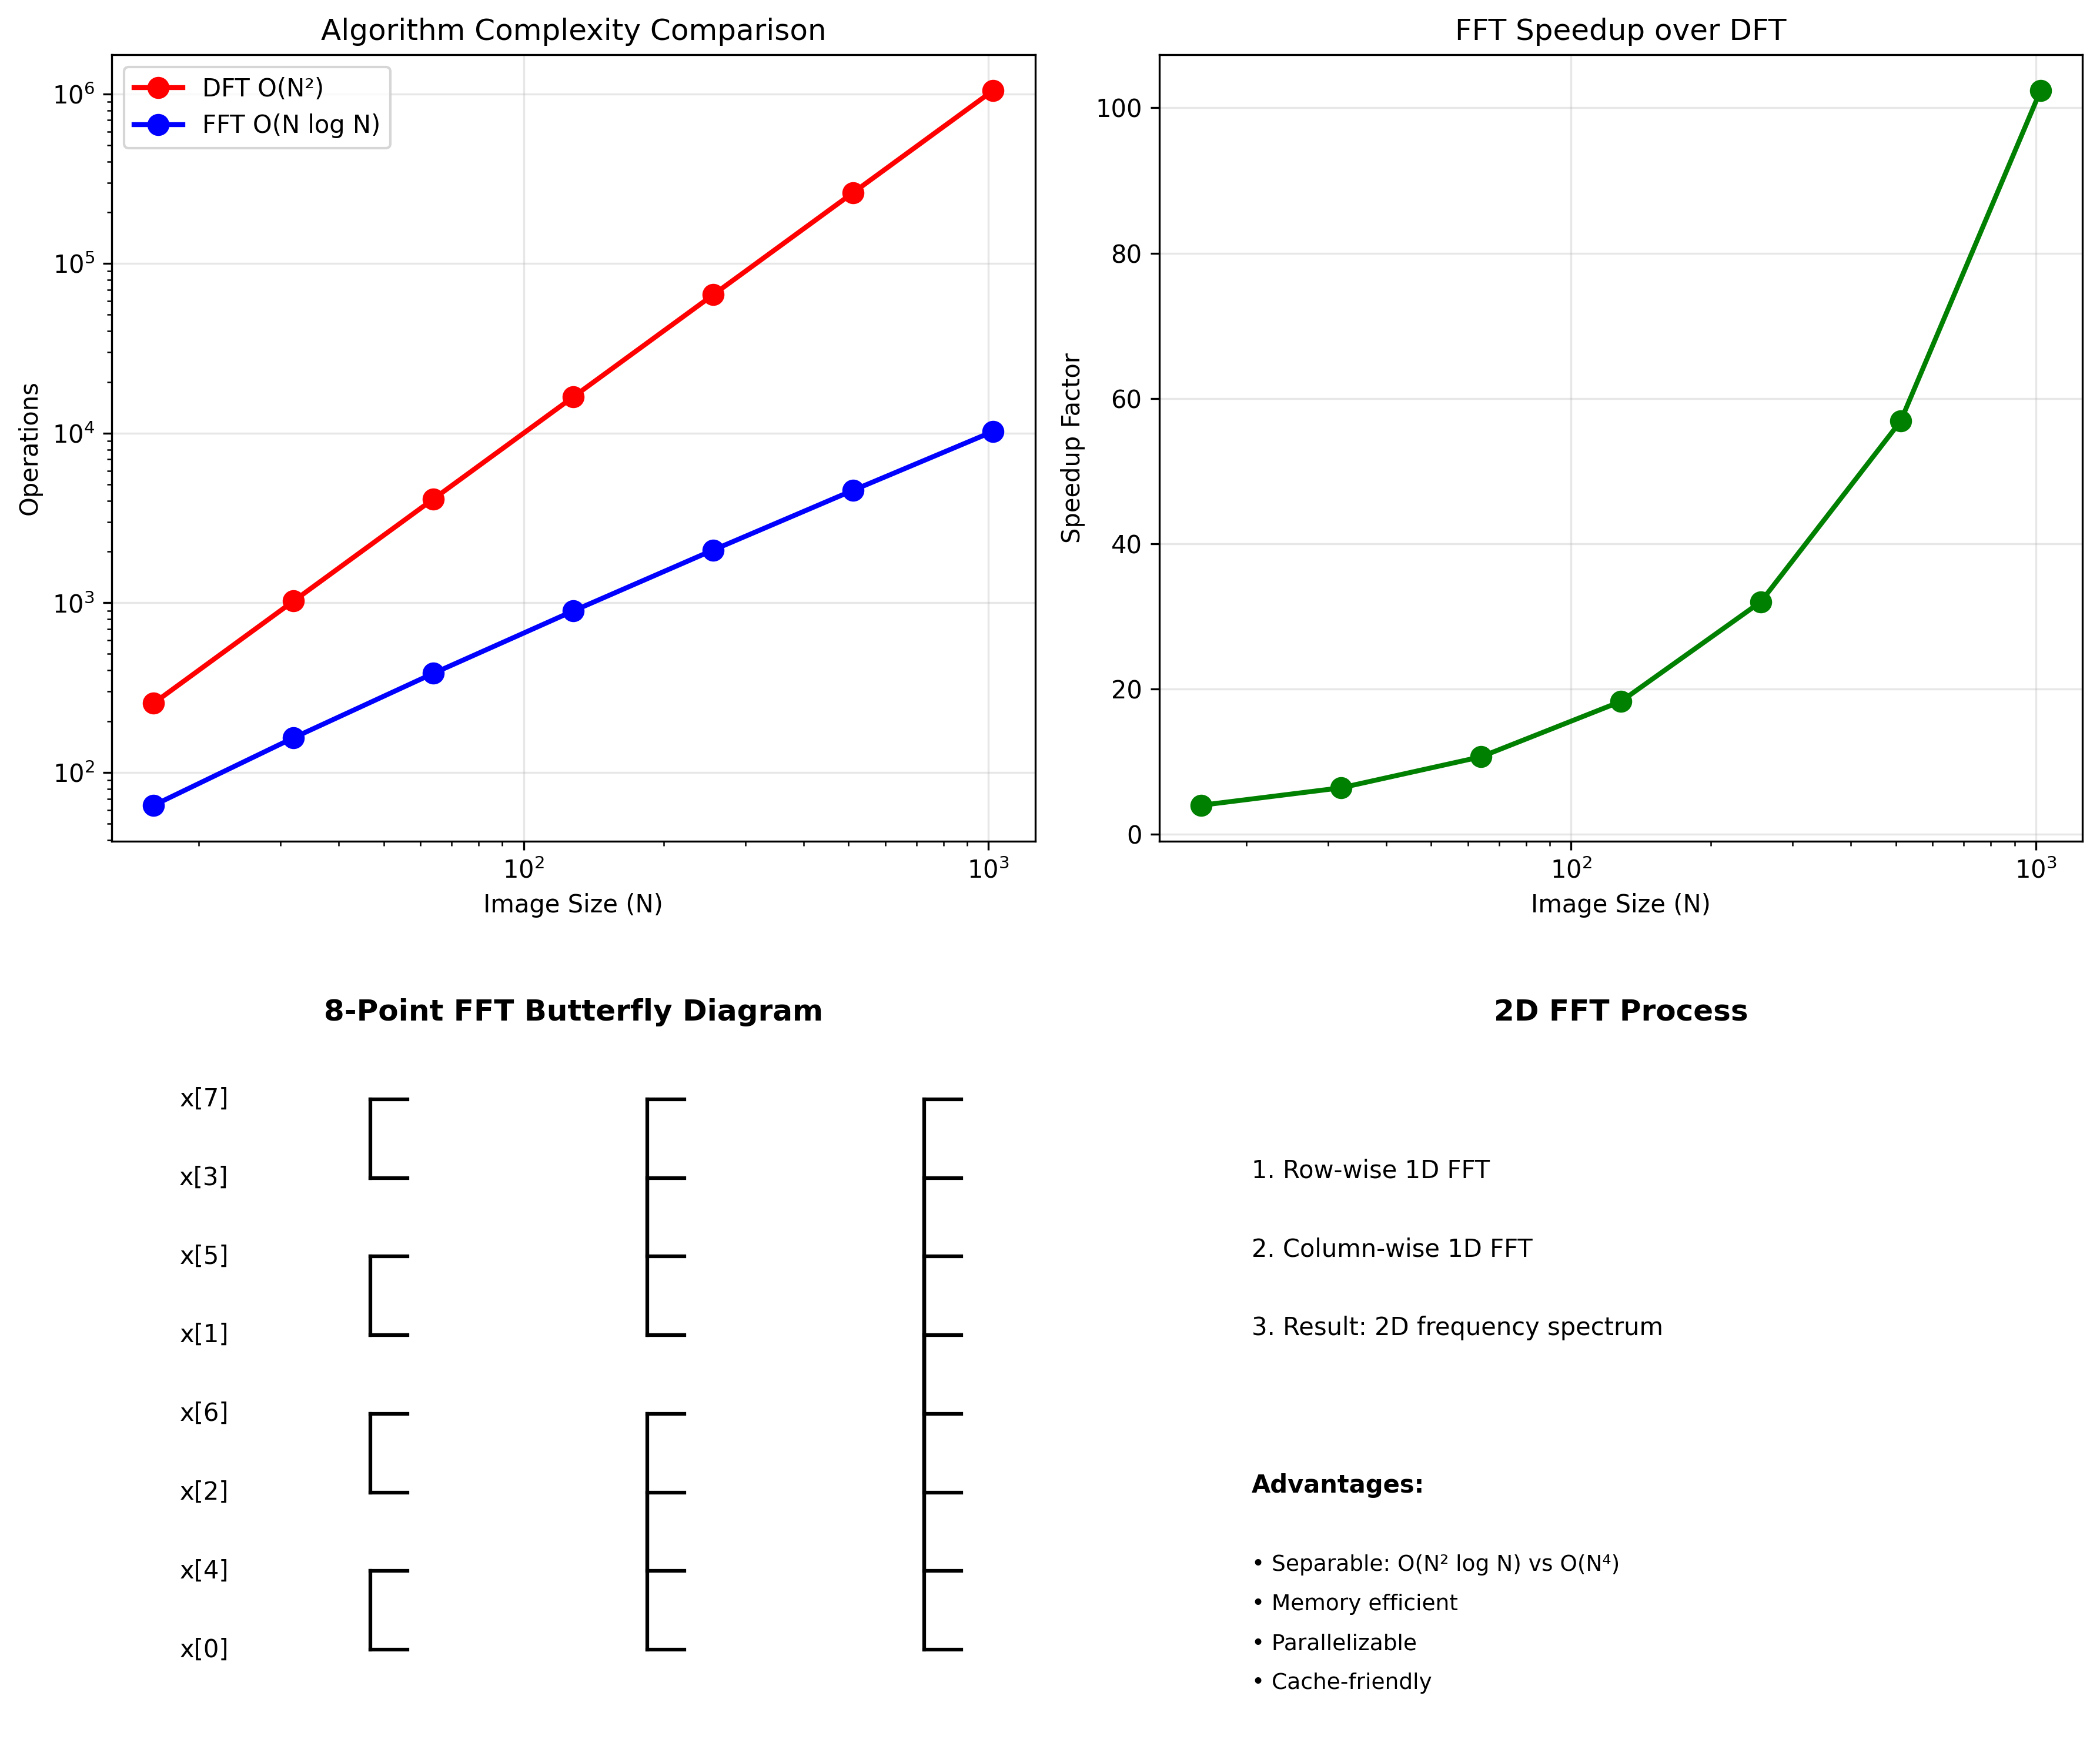
\includegraphics[width=\textwidth]{../figures/fft_algorithm.png}\\
\centering{\small FFT algorithm complexity comparison}
\end{columns}
\end{frame}

\section{Applications}

\begin{frame}{Periodic Noise Removal}
\begin{columns}
\begin{column}{0.45\textwidth}
\textbf{Problem:} Regular patterns in images due to:
\begin{itemize}
\item Electrical interference
\item Mechanical vibrations
\item Scanning artifacts
\item Aliasing effects
\end{itemize}

\textbf{Solution Approach:}
\begin{enumerate}
\item Analyze frequency spectrum
\item Identify periodic noise peaks
\item Design notch filters
\item Apply selective filtering
\end{enumerate}

\textbf{Notch Filter Design:}
$$H(u,v) = \prod_{k=1}^{Q} H_{Nk}(u,v) H_{N(-k)}(u,v)$$

Where $H_{Nk}$ removes frequency components at $(u_k, v_k)$
\end{column}
\begin{column}{0.5\textwidth}
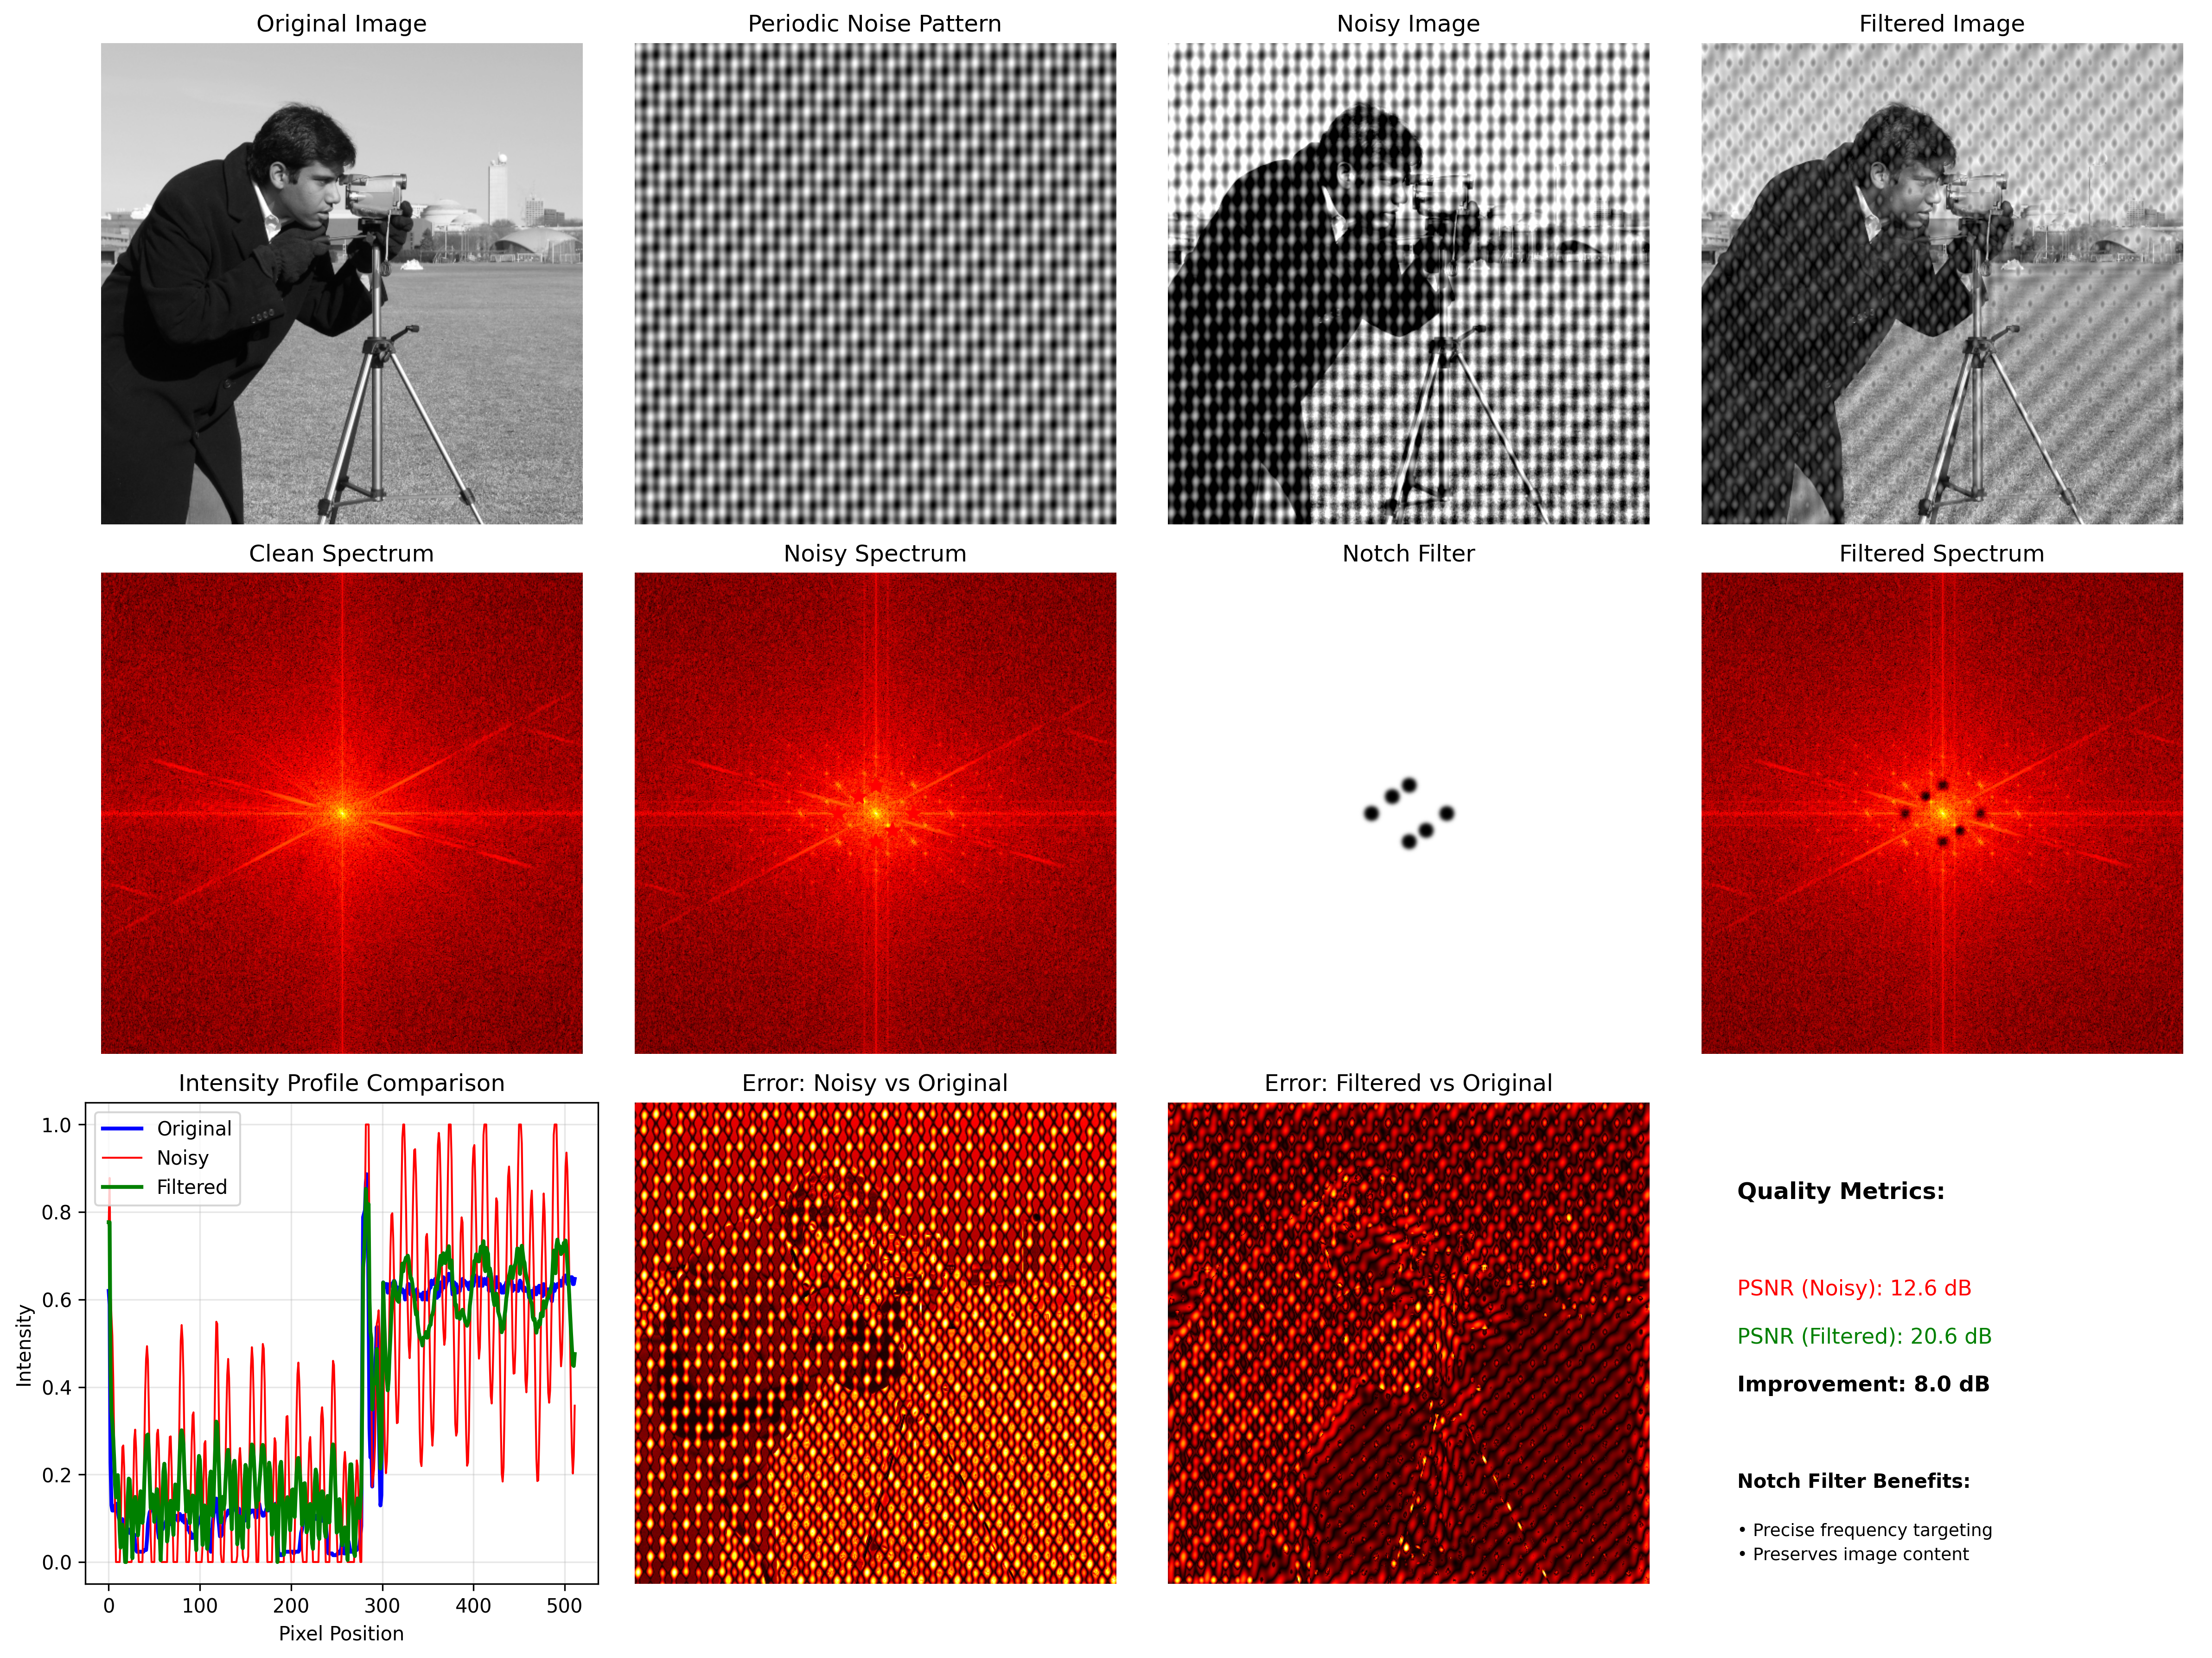
\includegraphics[width=\textwidth]{../figures/periodic_noise_removal.png}\\
\centering{\small Periodic noise identification and removal}
\end{column}
\end{columns}
\end{frame}

\begin{frame}{Image Sharpening in Frequency Domain}
\begin{columns}
\begin{column}{0.45\textwidth}
\textbf{High-Frequency Emphasis:}
$$H_{hfe}(u,v) = a + b \cdot H_{hp}(u,v)$$

Where $a \geq 0$, $b > 0$

\textbf{Advantages over Spatial Methods:}
\begin{itemize}
\item Direct frequency control
\item Flexible filter design
\item Efficient for large images
\item Multiple frequency bands
\end{itemize}

\textbf{Homomorphic Filtering:}
$$\ln[g(x,y)] = \ln[i(x,y)] + \ln[r(x,y)]$$

Separate illumination and reflectance in frequency domain:
\begin{enumerate}
\item $\ln$ transform
\item FFT
\item Filter design: $H(u,v)$
\item IFFT
\item Exponential
\end{enumerate}
\end{column}
\begin{column}{0.5\textwidth}
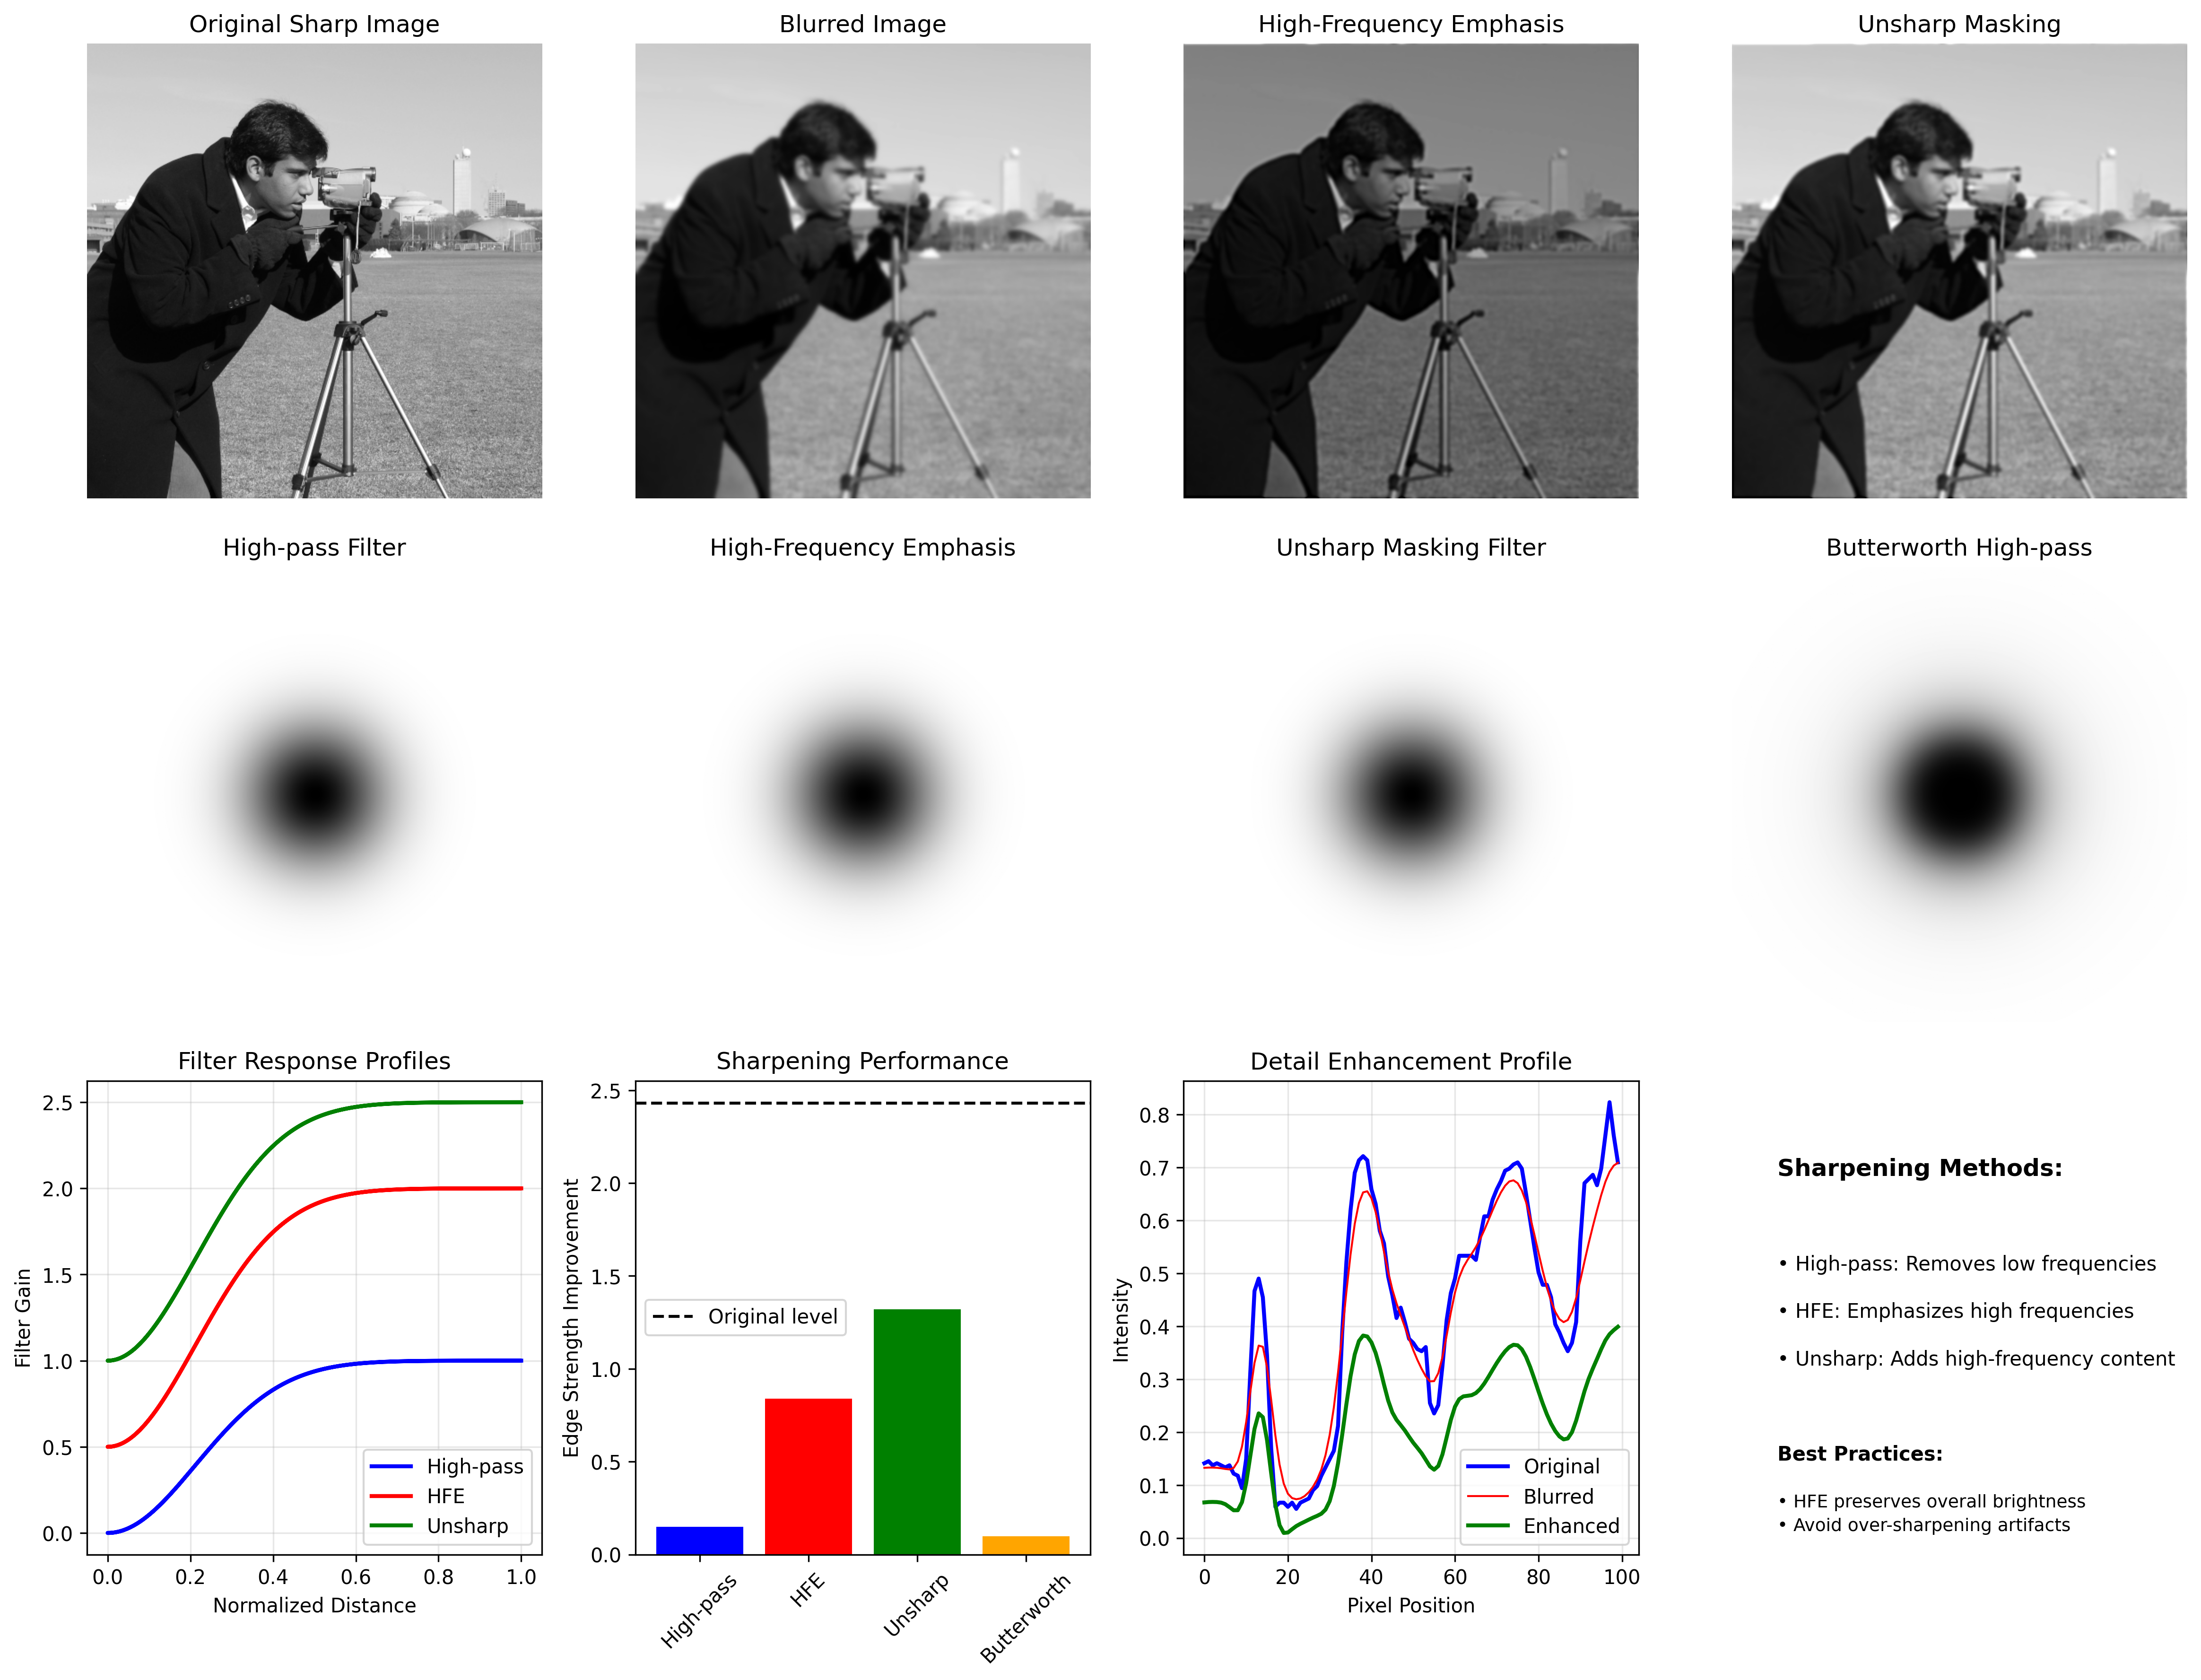
\includegraphics[width=\textwidth]{../figures/frequency_sharpening.png}\\
\centering{\small High-frequency emphasis and homomorphic filtering}
\end{column}
\end{columns}
\end{frame}

\begin{frame}{Medical Image Enhancement}
\begin{columns}
\begin{column}{0.45\textwidth}
\textbf{Applications in Medical Imaging:}
\begin{itemize}
\item X-ray image enhancement
\item MRI noise reduction
\item Ultrasound speckle removal
\item CT artifact correction
\end{itemize}

\textbf{Frequency Domain Benefits:}
\begin{itemize}
\item Precise noise frequency targeting
\item Preservation of diagnostic features
\item Quantitative filter specification
\item Minimal spatial artifacts
\end{itemize}

\textbf{Example: X-ray Enhancement}
\begin{enumerate}
\item Identify noise frequencies
\item Design adaptive filters
\item Apply frequency-selective enhancement
\item Preserve bone/tissue contrast
\end{enumerate}
\end{column}
\begin{column}{0.5\textwidth}
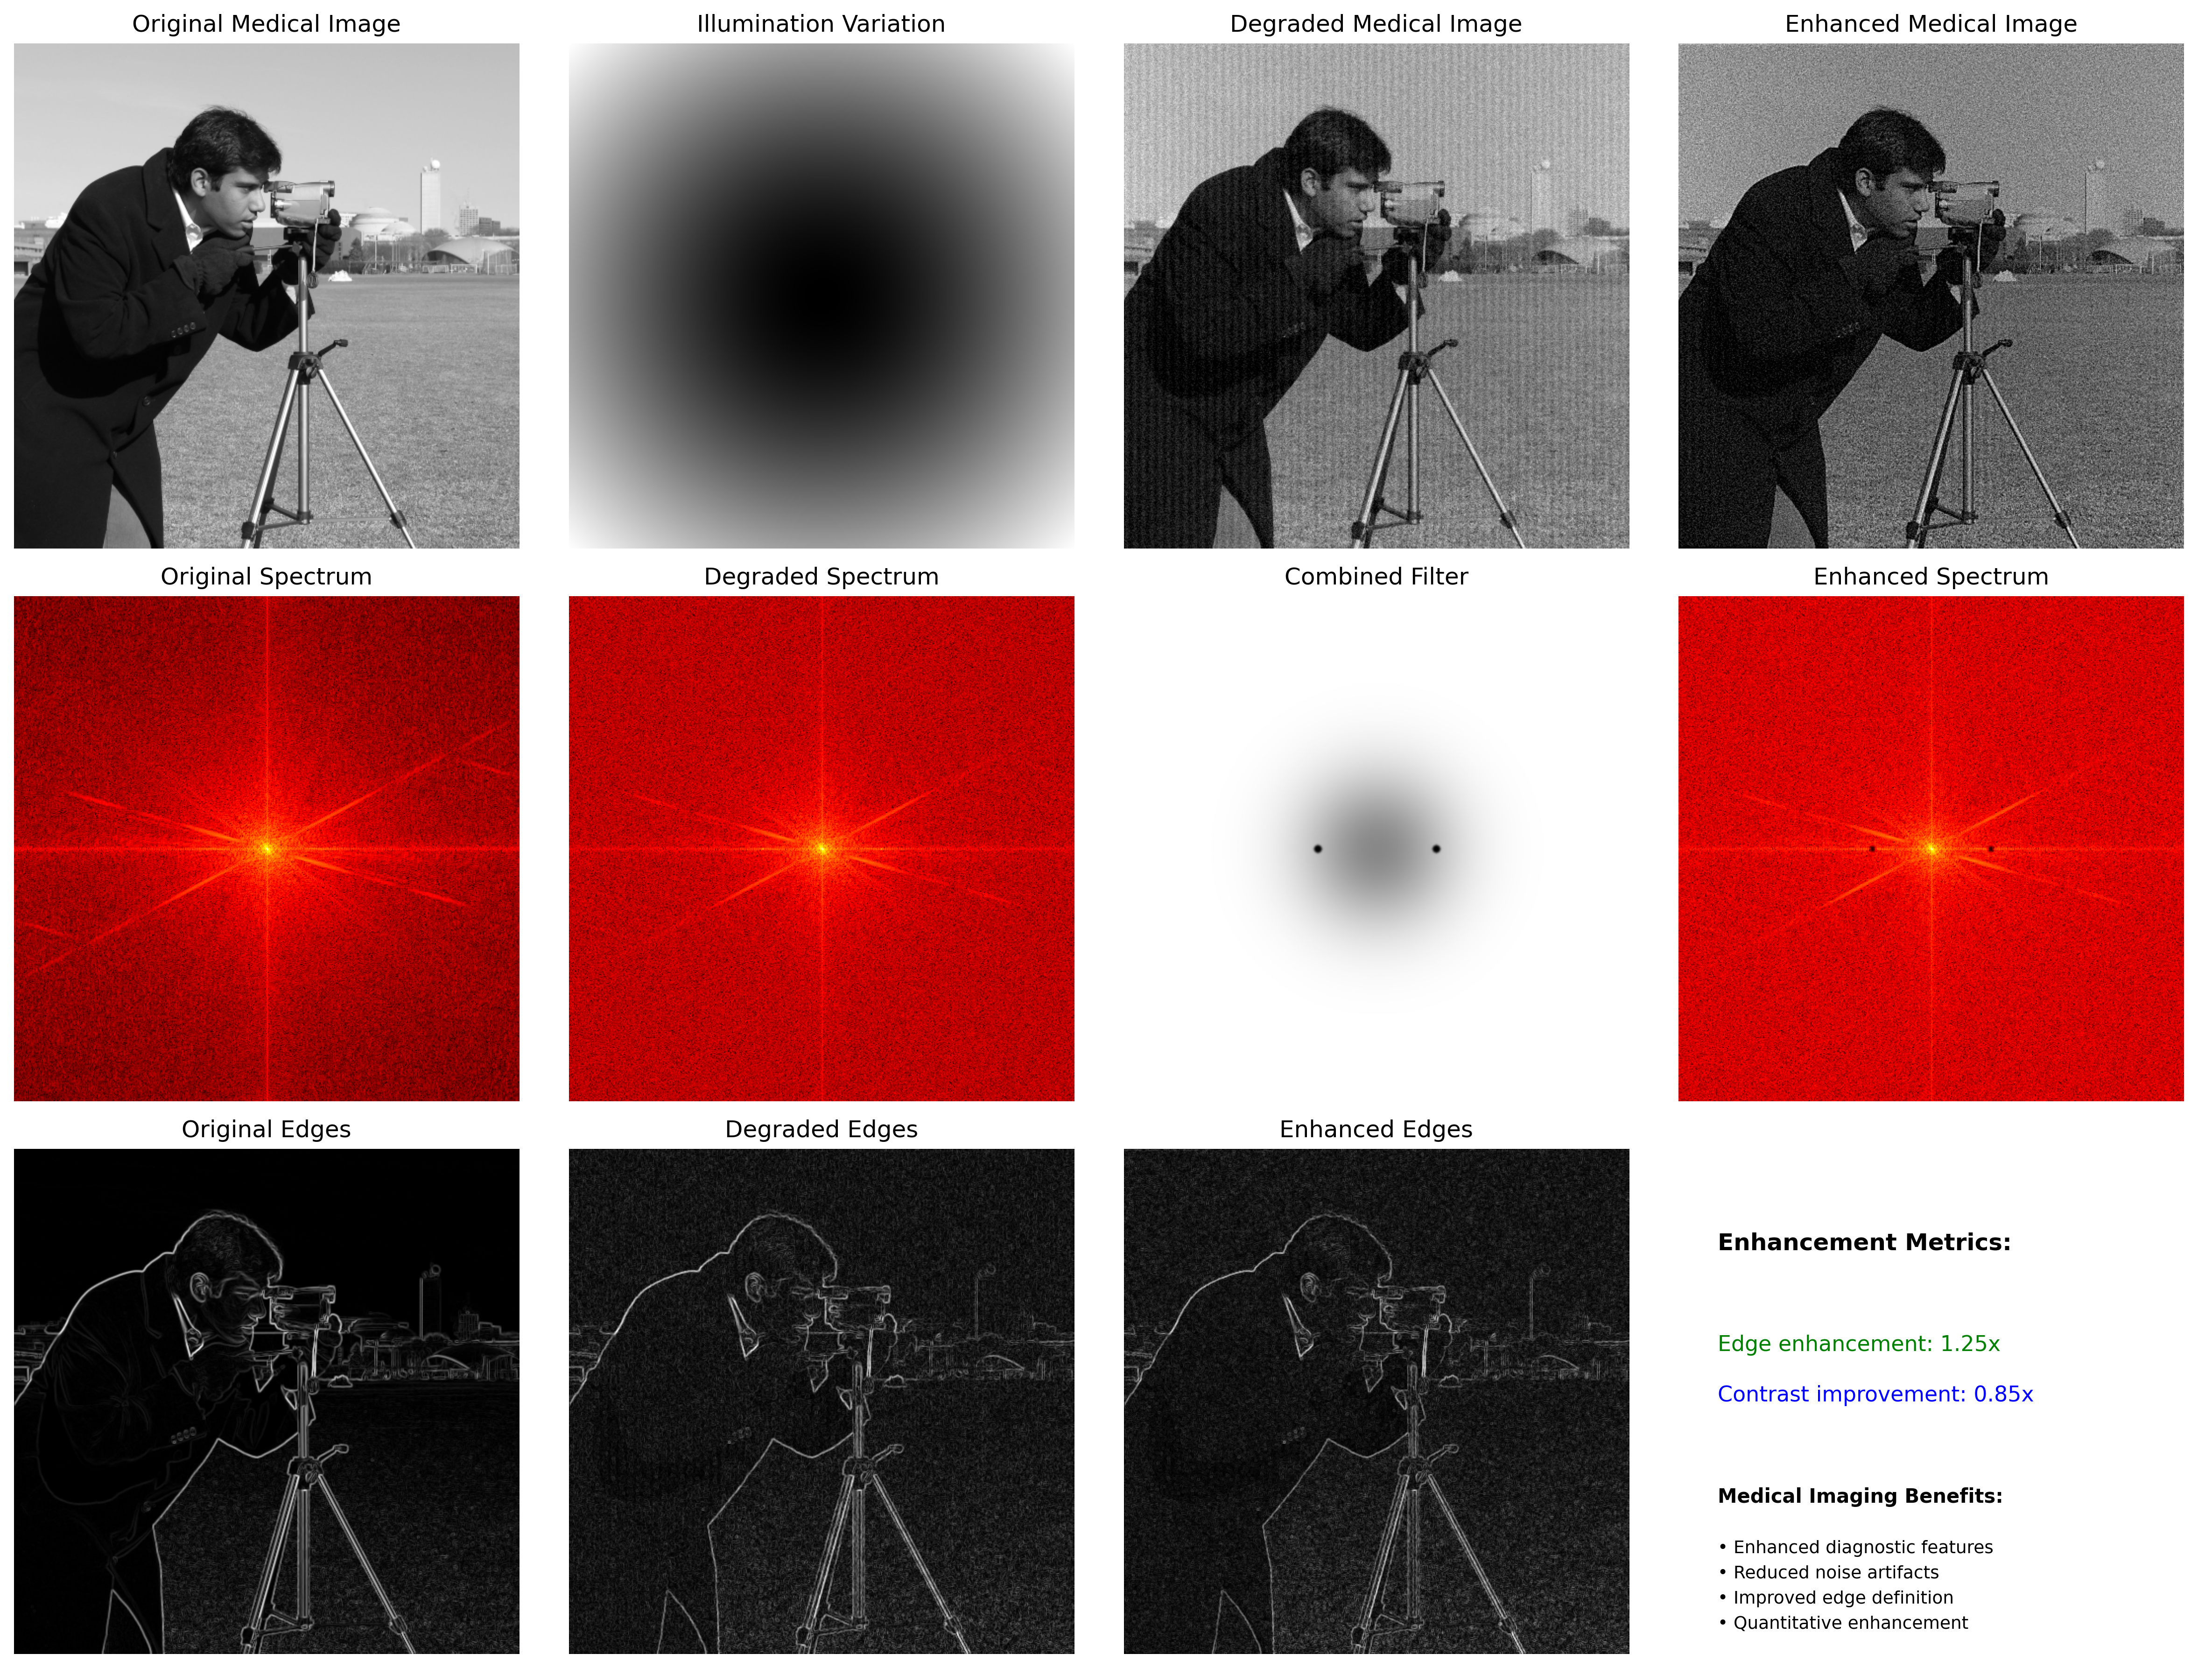
\includegraphics[width=\textwidth]{../figures/medical_frequency_enhancement.png}\\
\centering{\small Medical image frequency domain enhancement}
\end{column}
\end{columns}
\end{frame}

\begin{frame}{Satellite and Remote Sensing}
\begin{columns}
\begin{column}{0.45\textwidth}
\textbf{Remote Sensing Challenges:}
\begin{itemize}
\item Atmospheric distortion
\item Sensor noise patterns
\item Periodic interference
\item Multi-spectral alignment
\end{itemize}

\textbf{Frequency Domain Solutions:}
\begin{itemize}
\item Atmospheric correction filters
\item Sensor pattern noise removal
\item Radiometric enhancement
\item Spectral band optimization
\end{itemize}

\textbf{Preprocessing Pipeline:}
\begin{enumerate}
\item Radiometric calibration
\item Frequency domain denoising
\item Atmospheric correction
\item Multi-spectral registration
\item Feature enhancement
\end{enumerate}
\end{column}
\begin{column}{0.5\textwidth}
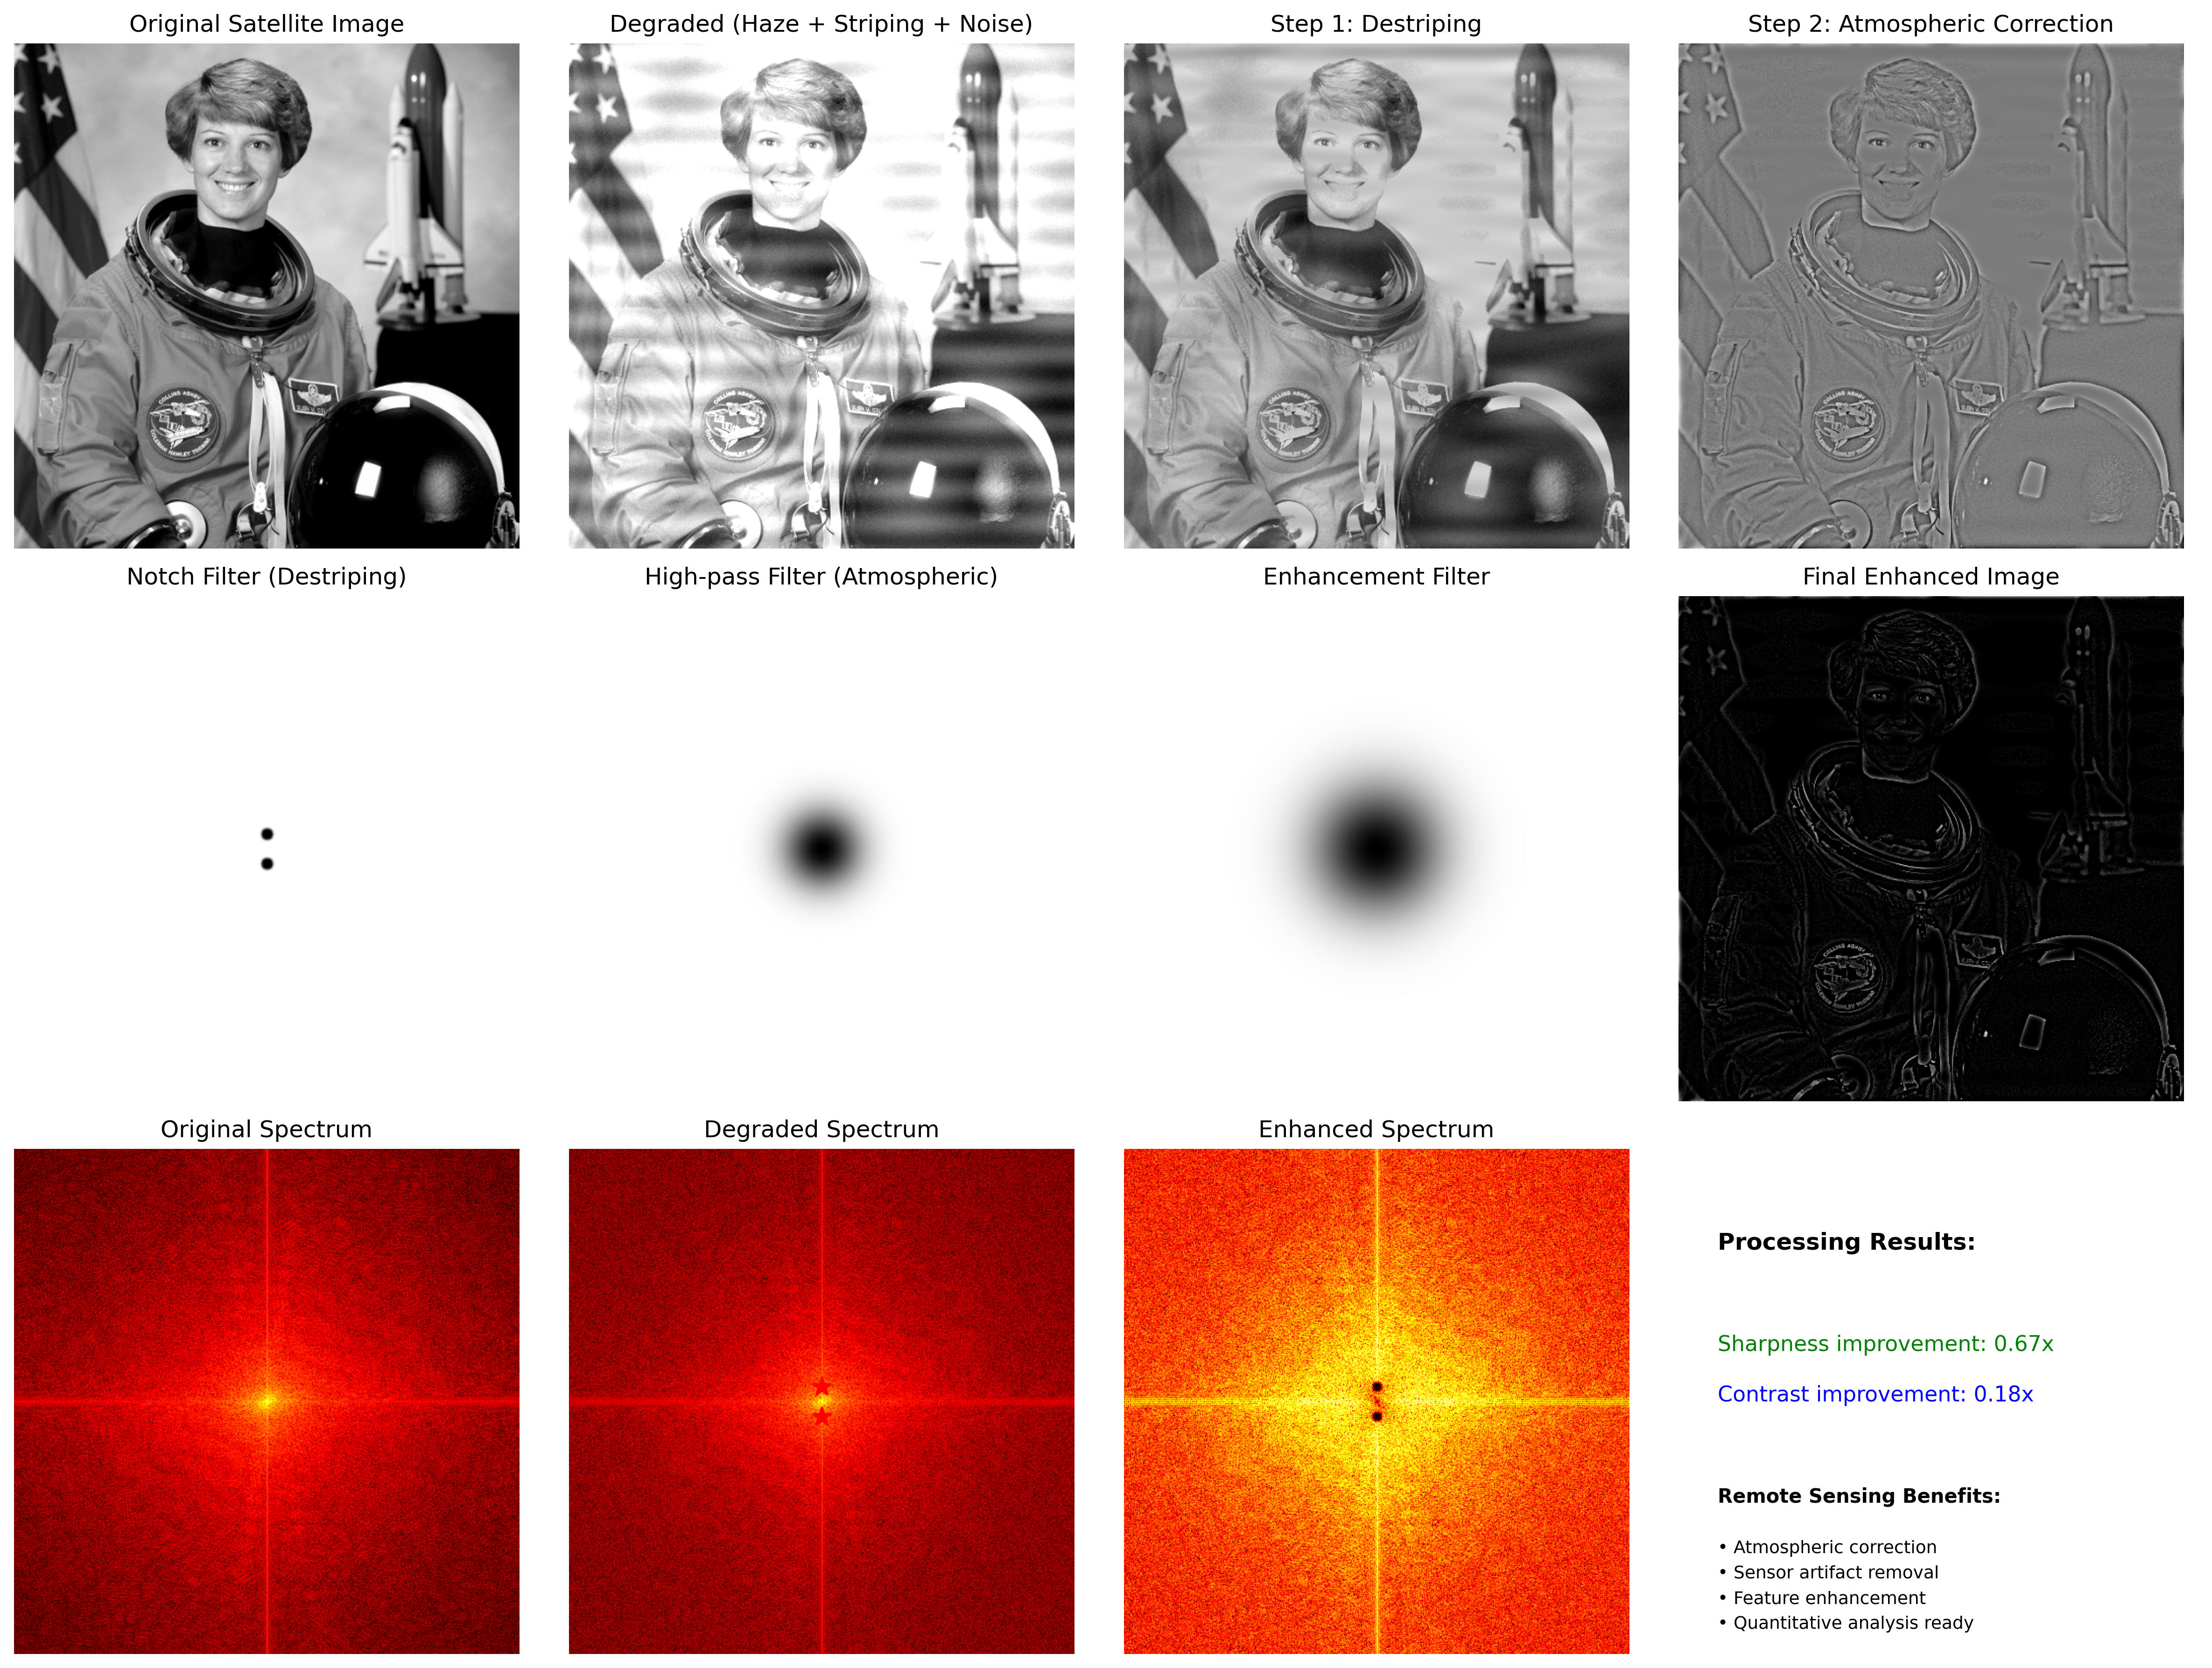
\includegraphics[width=\textwidth]{../figures/satellite_frequency_processing.png}\\
\centering{\small Satellite image frequency domain processing}
\end{column}
\end{columns}
\end{frame}

\section{Advanced Topics}

\begin{frame}{Homomorphic Filtering}
\begin{columns}
\begin{column}{0.55\textwidth}
\textbf{Illumination-Reflectance Model:}
$$f(x,y) = i(x,y) \cdot r(x,y)$$

Where:
\begin{itemize}
\item $i(x,y)$ = illumination component (low frequency)
\item $r(x,y)$ = reflectance component (high frequency)
\end{itemize}

\textbf{Logarithmic Transformation:}
$$z(x,y) = \ln[f(x,y)] = \ln[i(x,y)] + \ln[r(x,y)]$$

\textbf{Frequency Domain Processing:}
$$Z(u,v) = I(u,v) + R(u,v)$$

\textbf{Homomorphic Filter:}
$$H(u,v) = (\gamma_H - \gamma_L)\left[1 - e^{-c[\frac{D^2(u,v)}{D_0^2}]}\right] + \gamma_L$$

Where $\gamma_L < 1$ (compress illumination), $\gamma_H > 1$ (enhance reflectance)
\end{column}
\begin{column}{0.4\textwidth}
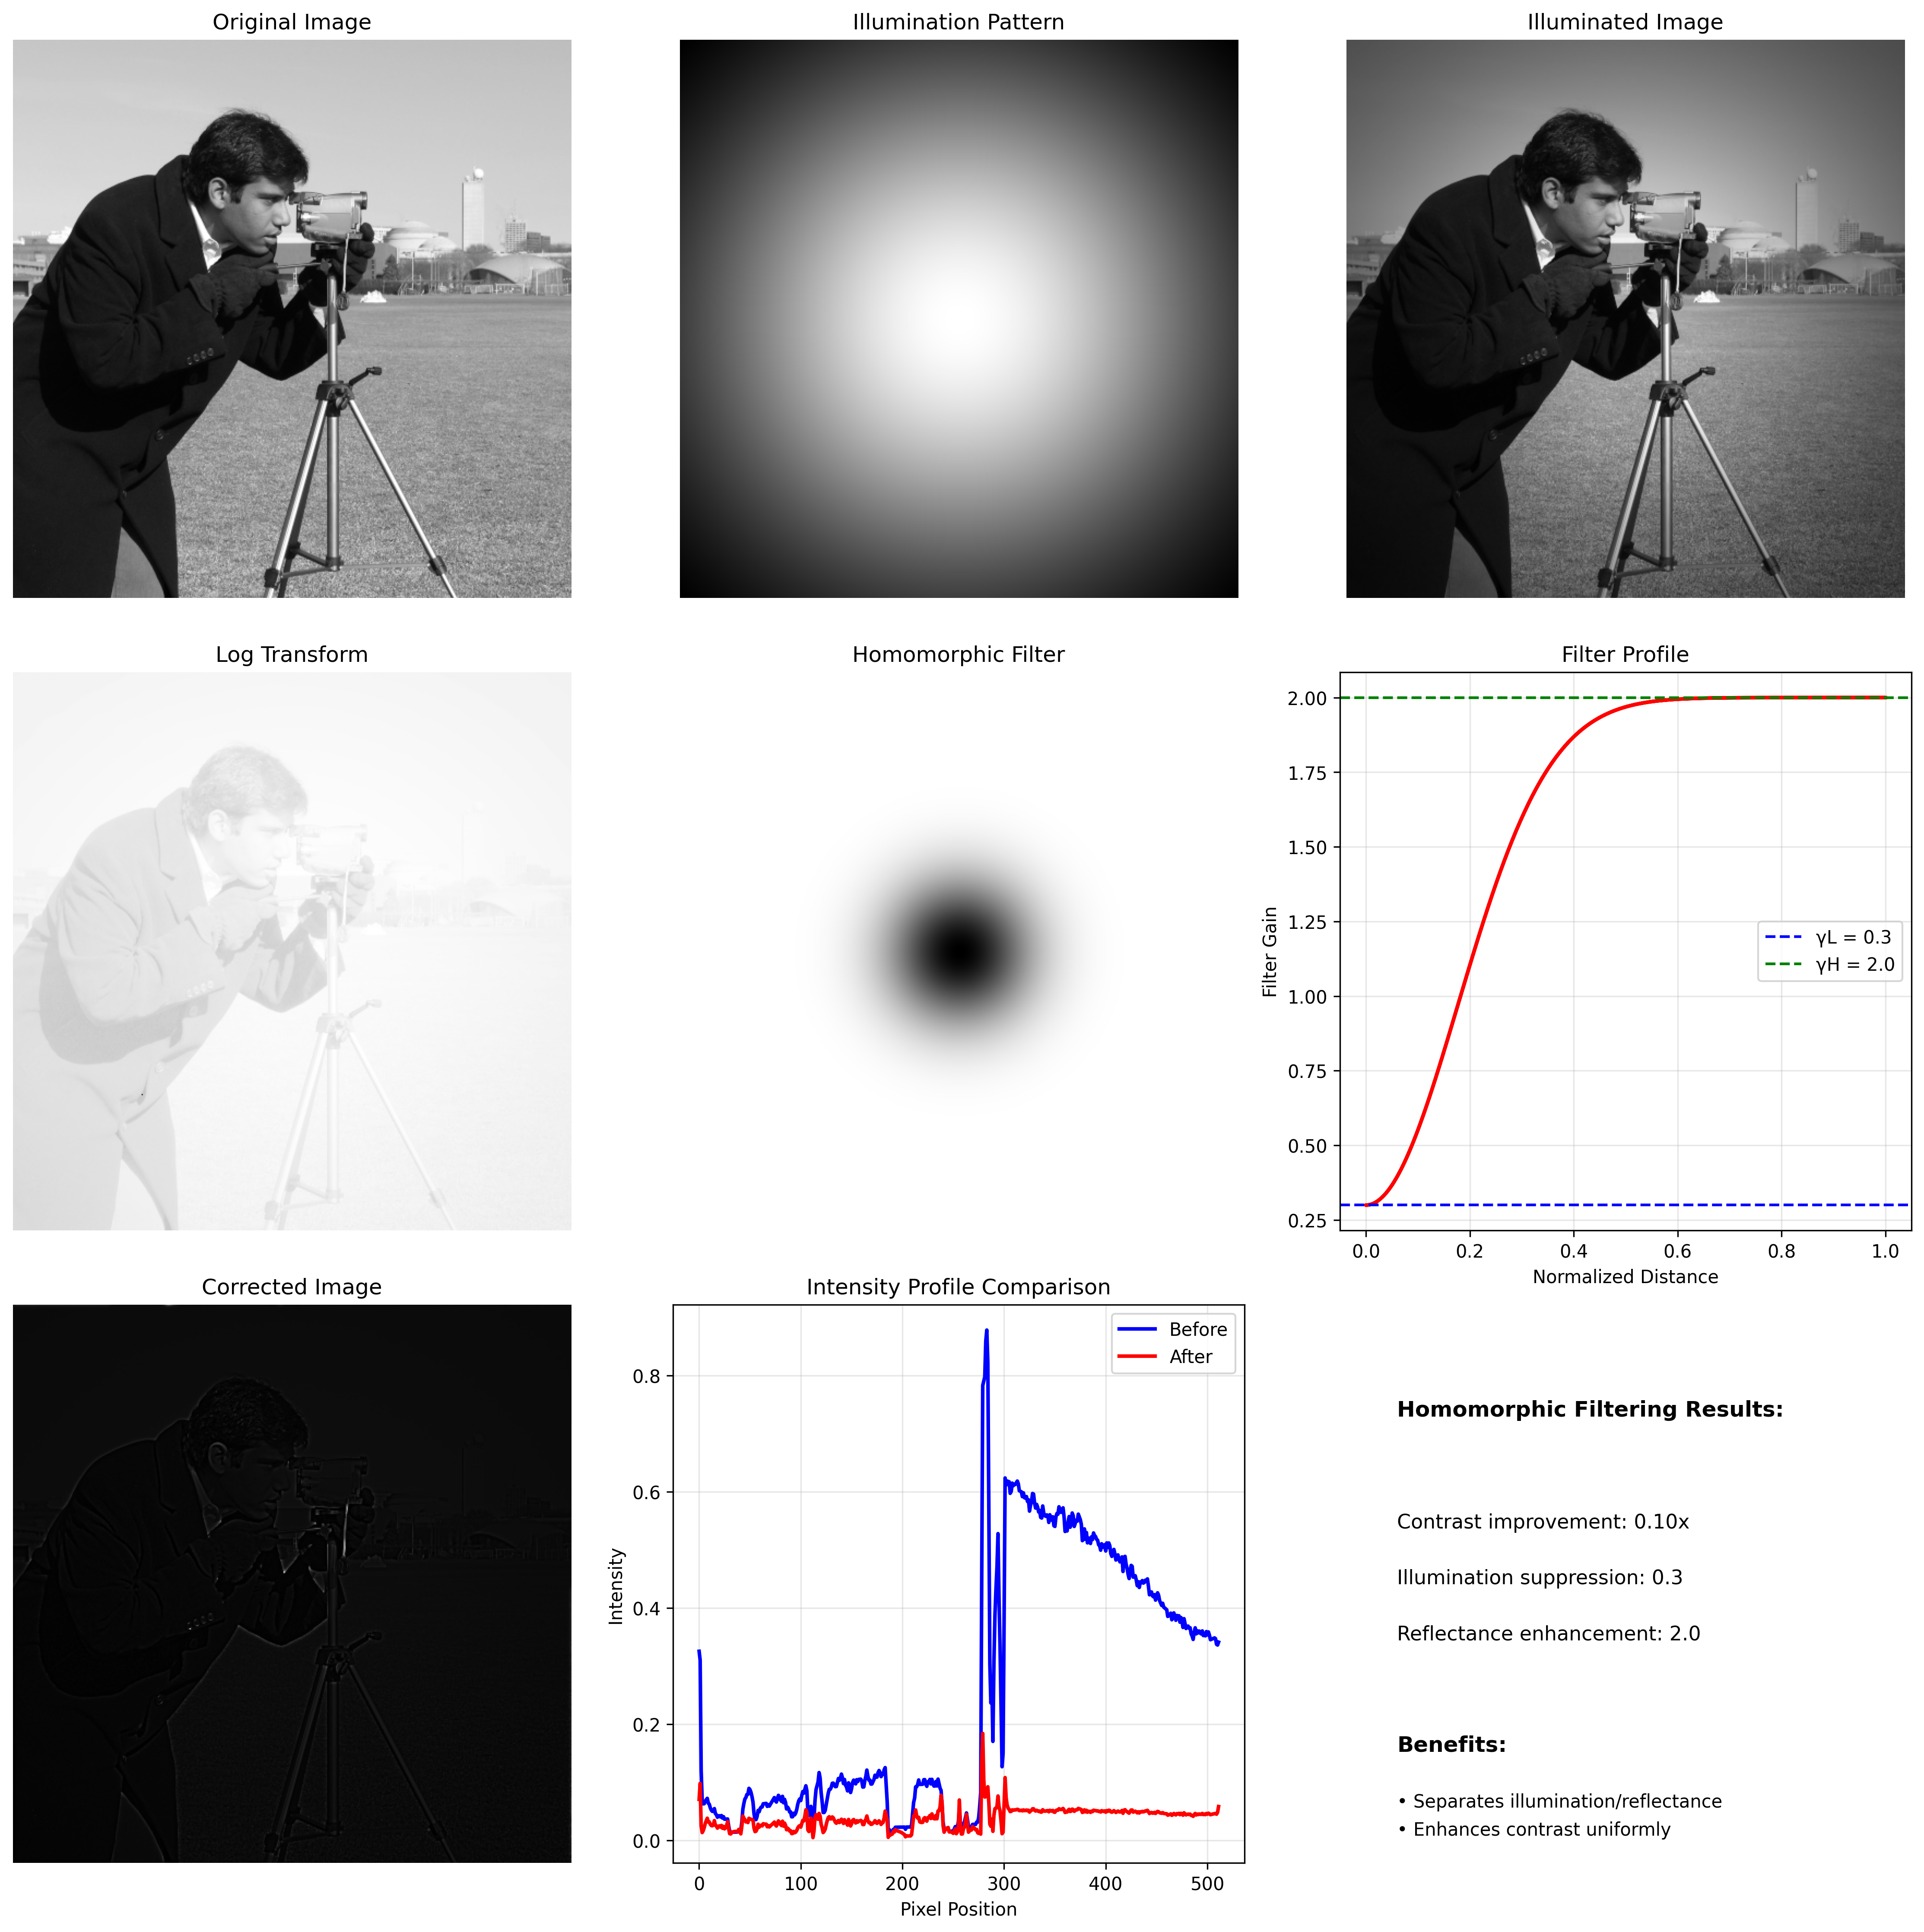
\includegraphics[width=\textwidth]{../figures/homomorphic_filtering.png}\\
\centering{\small Homomorphic filtering process and results}
\end{column}
\end{columns}
\end{frame}

\begin{frame}{Wiener Filtering}
\begin{columns}
\begin{column}{0.55\textwidth}
\textbf{Degradation Model:}
$$g(x,y) = h(x,y) * f(x,y) + n(x,y)$$

In frequency domain:
$$G(u,v) = H(u,v)F(u,v) + N(u,v)$$

\textbf{Wiener Filter:}
$$\hat{F}(u,v) = \left[\frac{H^*(u,v)}{|H(u,v)|^2 + \frac{S_n(u,v)}{S_f(u,v)}}\right] G(u,v)$$

Where:
\begin{itemize}
\item $H^*(u,v)$ = complex conjugate of degradation
\item $S_n(u,v)$ = noise power spectrum
\item $S_f(u,v)$ = original image power spectrum
\end{itemize}

\textbf{Simplified Form (constant ratio):}
$$\hat{F}(u,v) = \frac{H^*(u,v)}{|H(u,v)|^2 + K} G(u,v)$$
\end{column}
\begin{column}{0.4\textwidth}
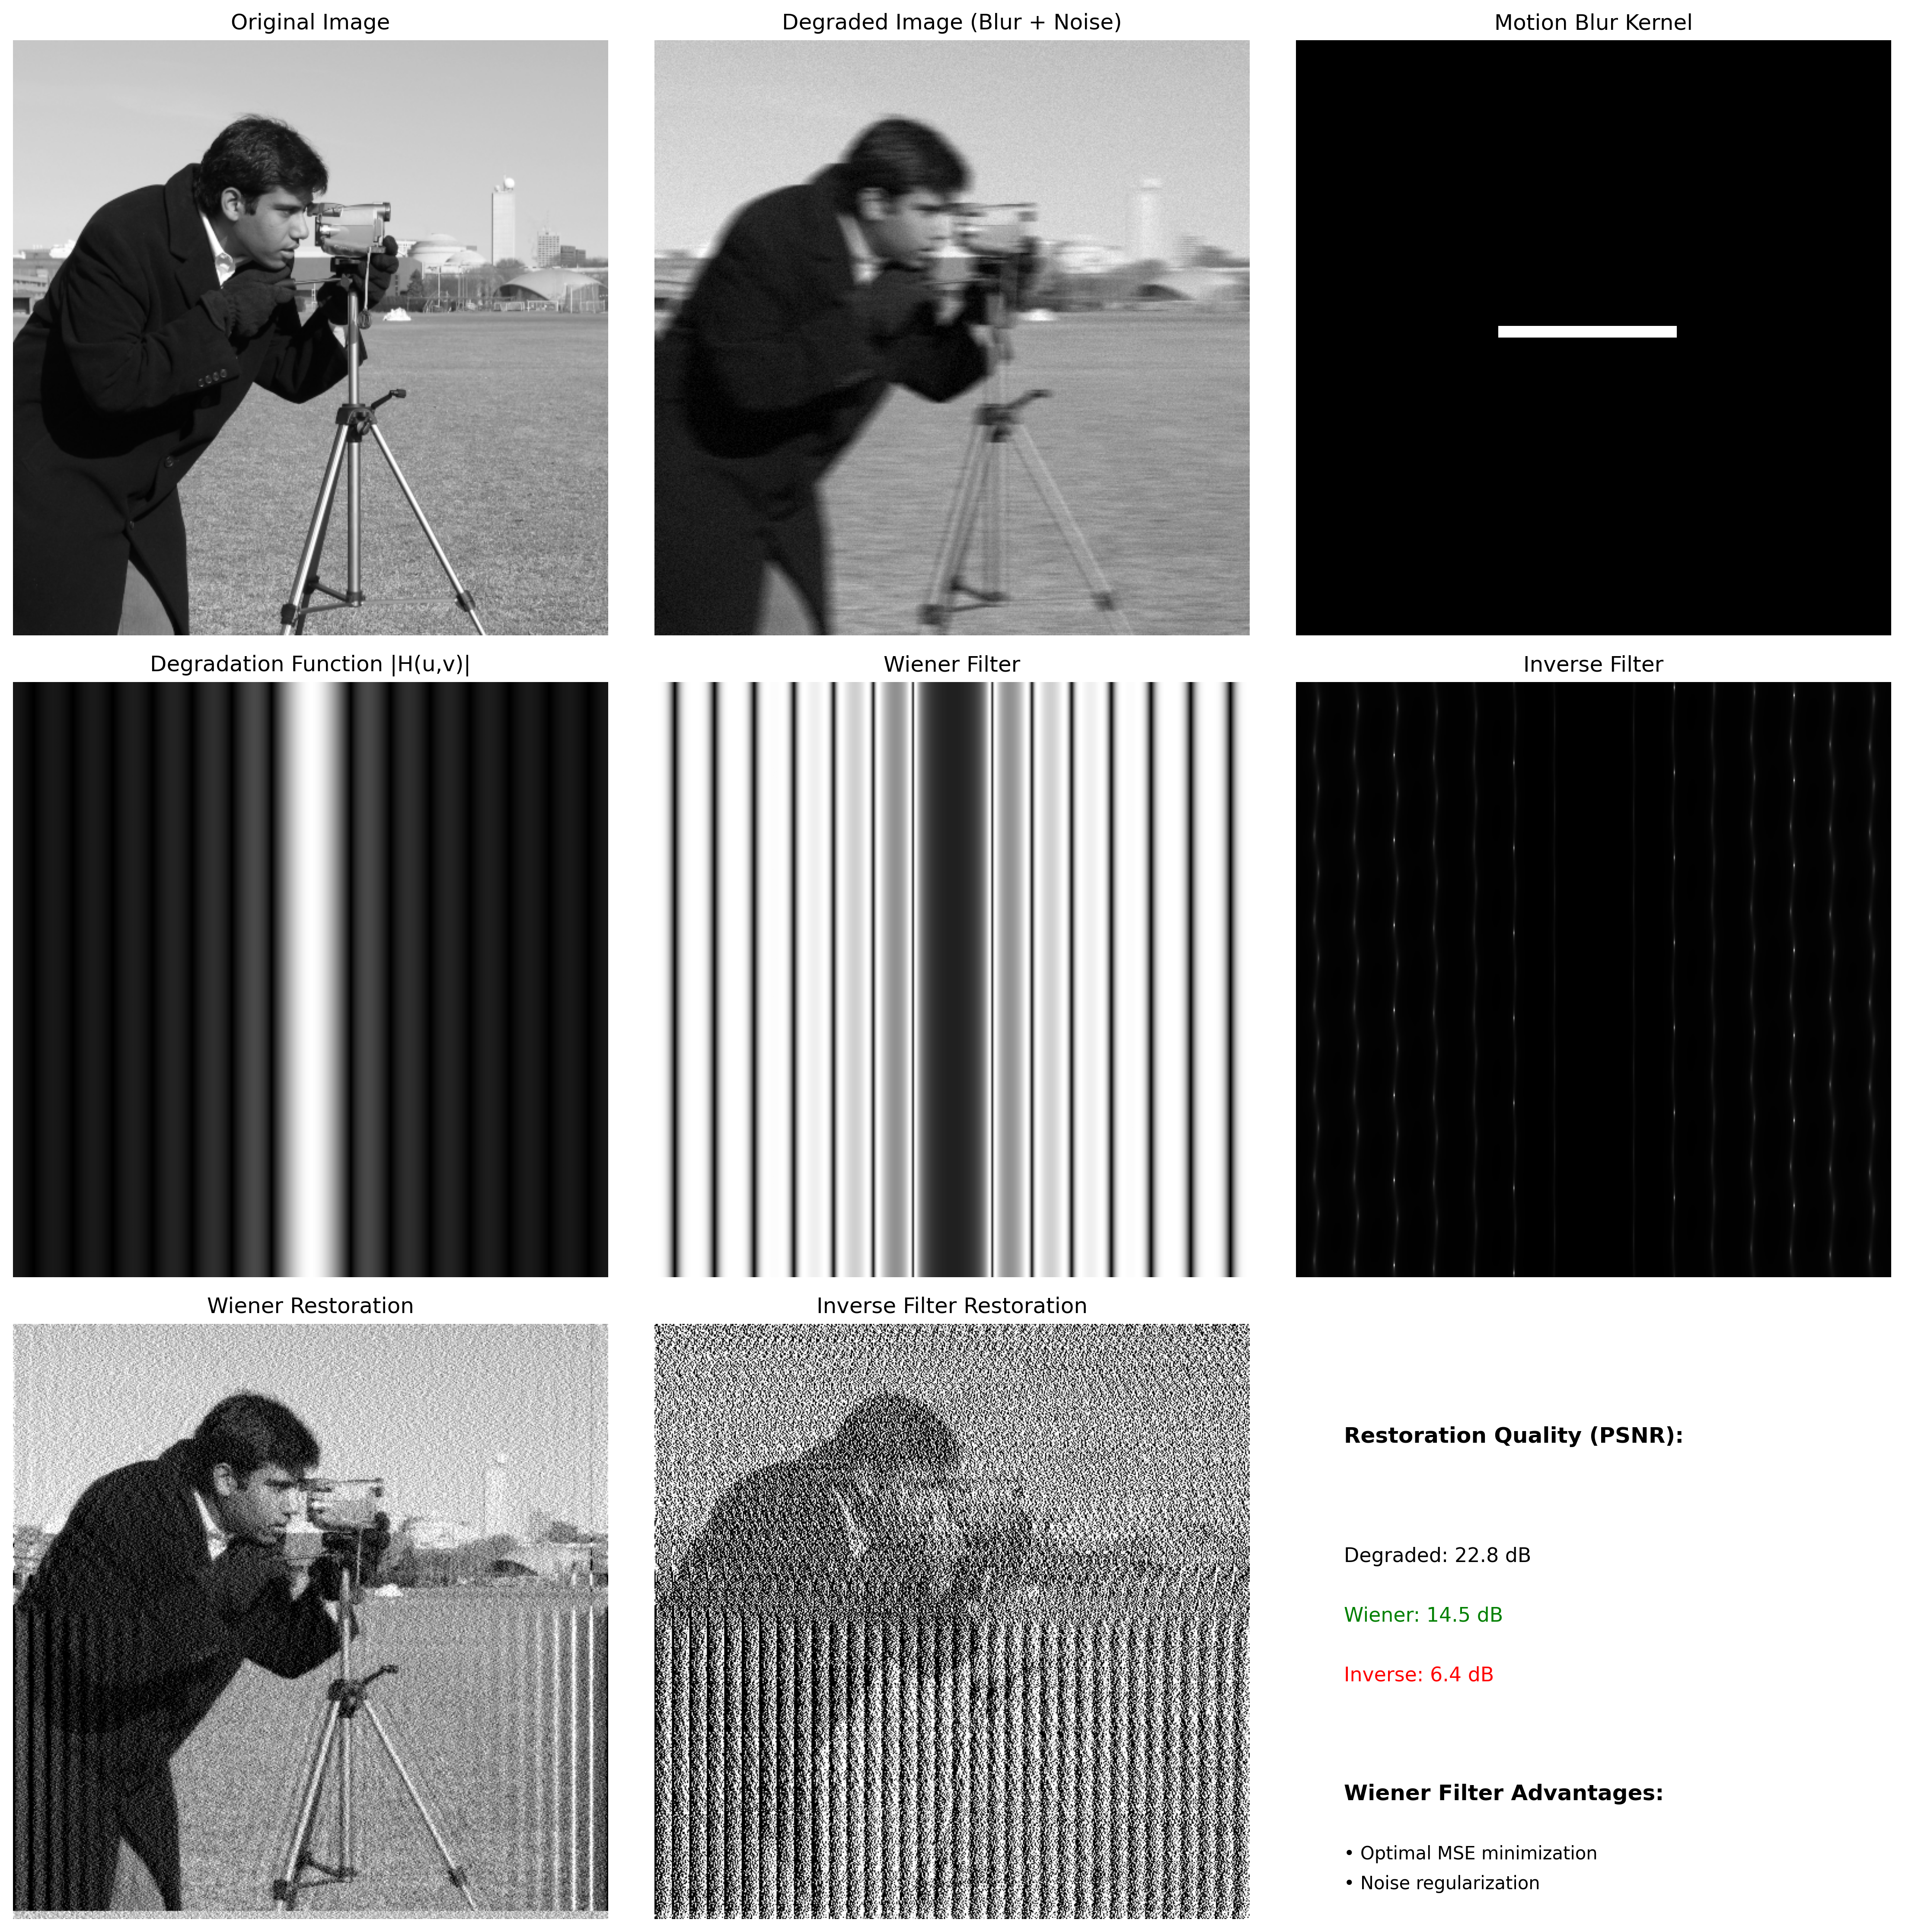
\includegraphics[width=\textwidth]{../figures/wiener_filtering.png}\\
\centering{\small Wiener filter restoration results}
\end{column}
\end{columns}
\end{frame}

\begin{frame}{Selective Filtering and Masking}
\begin{columns}
\begin{column}{0.55\textwidth}
\textbf{Selective Frequency Removal:}

\textbf{Interactive Frequency Editing:}
\begin{enumerate}
\item Display magnitude spectrum
\item Identify unwanted frequencies
\item Create binary masks
\item Apply selective filtering
\end{enumerate}

\textbf{Automated Detection:}
$$\text{Peak}(u,v) = \begin{cases}
1 & \text{if } |F(u,v)| > T \cdot \text{median}(|F|) \\
0 & \text{otherwise}
\end{cases}$$

\textbf{Morphological Mask Refinement:}
\begin{itemize}
\item Dilation for connected components
\item Erosion for noise removal
\item Gaussian smoothing for gradual transitions
\end{itemize}

\textbf{Quality Preservation:}
$$H_{smooth}(u,v) = H_{binary}(u,v) * G_{\sigma}(u,v)$$
\end{column}
\begin{column}{0.4\textwidth}
\includegraphics[width=\textwidth]{../figures/selective_filtering.png}\\
\centering{\small Selective frequency masking and removal}
\end{column}
\end{columns}
\end{frame}

\begin{frame}{Multi-Scale Frequency Analysis}
\begin{columns}
\begin{column}{0.55\textwidth}
\textbf{Wavelet Transform Integration:}

\textbf{Short-Time Fourier Transform (STFT):}
$$F(u,v,x_0,y_0) = \int \int f(x,y)w(x-x_0,y-y_0)e^{-j2\pi(ux+vy)}dxdy$$

\textbf{Gabor Filtering:}
$$h(x,y) = g(x,y) \cdot e^{j2\pi(u_0x + v_0y)}$$

Where $g(x,y)$ is a Gaussian window.

\textbf{Multi-Resolution Processing:}
\begin{enumerate}
\item Decompose into frequency bands
\item Process each band independently
\item Apply scale-specific enhancements
\item Reconstruct enhanced image
\end{enumerate}

\textbf{Adaptive Frequency Enhancement:}
$$H_{adaptive}(u,v) = f(\text{local variance}, \text{edge strength})$$
\end{column}
\begin{column}{0.4\textwidth}
\includegraphics[width=\textwidth]{../figures/multiscale_frequency.png}\\
\centering{\small Multi-scale frequency domain analysis}
\end{column}
\end{columns}
\end{frame}

\section{Best Practices}

\begin{frame}{Common Pitfalls and Solutions}
\begin{alertblock}{Pitfall 1: Ringing Artifacts}
\textbf{Problem:} Ideal filters cause oscillations near edges
\textbf{Solution:} Use smooth filters (Gaussian, Butterworth)
\end{alertblock}

\begin{alertblock}{Pitfall 2: Frequency Leakage}
\textbf{Problem:} Abrupt image boundaries create artifacts
\textbf{Solution:} Apply windowing or image padding
\end{alertblock}

\begin{alertblock}{Pitfall 3: Phase Distortion}
\textbf{Problem:} Incorrect phase handling destroys spatial relationships
\textbf{Solution:} Use zero-phase filters or preserve phase information
\end{alertblock}

\begin{alertblock}{Pitfall 4: Over-filtering}
\textbf{Problem:} Excessive filtering removes important details
\textbf{Solution:} Analyze frequency content before designing filters
\end{alertblock}
\end{frame}

\begin{frame}{Filter Design Guidelines}
\textbf{Frequency Domain Filter Design Process:}

\begin{columns}
\column{0.5\textwidth}
\textbf{1. Analysis Phase:}
\begin{itemize}
\item Examine frequency spectrum
\item Identify noise characteristics
\item Determine desired enhancements
\item Assess phase sensitivity
\end{itemize}

\textbf{2. Design Phase:}
\begin{itemize}
\item Choose filter type and parameters
\item Consider transition smoothness
\item Account for computational constraints
\item Design for minimal artifacts
\end{itemize}

\column{0.45\textwidth}
\textbf{3. Implementation Phase:}
\begin{itemize}
\item Apply proper preprocessing
\item Handle boundary conditions
\item Monitor for artifacts
\item Validate results quantitatively
\end{itemize}

\textbf{4. Optimization Phase:}
\begin{itemize}
\item Fine-tune parameters
\item Compare with spatial methods
\item Evaluate computational efficiency
\item Document optimal settings
\end{itemize}
\end{columns}

\textbf{Filter Selection Criteria:}
\begin{itemize}
\item \textbf{Smoothness:} Gaussian > Butterworth > Ideal
\item \textbf{Computational cost:} Ideal < Butterworth < Gaussian
\item \textbf{Artifact control:} Gaussian > Butterworth > Ideal
\end{itemize}
\end{frame}

\begin{frame}{Quality Assessment}
\begin{columns}
\begin{column}{0.5\textwidth}
\textbf{Quantitative Metrics:}

\textbf{Frequency Domain Metrics:}
\begin{align}
\text{SNR}_{freq} &= 10\log_{10}\frac{\sum |F_{signal}|^2}{\sum |F_{noise}|^2} \\
\text{Spectral Flatness} &= \frac{\text{geometric mean}}{\text{arithmetic mean}}
\end{align}

\textbf{Spatial Domain Validation:}
\begin{align}
\text{PSNR} &= 20\log_{10}\frac{255}{\sqrt{\text{MSE}}} \\
\text{SSIM} &= \frac{(2\mu_x\mu_y + c_1)(2\sigma_{xy} + c_2)}{(\mu_x^2 + \mu_y^2 + c_1)(\sigma_x^2 + \sigma_y^2 + c_2)}
\end{align}

\textbf{Artifact Detection:}
\begin{itemize}
\item Ringing analysis near edges
\item Frequency leakage assessment
\item Phase coherence evaluation
\end{itemize}
\end{column}
\begin{column}{0.45\textwidth}
\includegraphics[width=\textwidth]{../figures/quality_assessment.png}\\
\centering{\small Quality metrics for frequency domain enhancement}
\end{column}
\end{columns}
\end{frame}

\begin{frame}{Computational Considerations}
\textbf{Performance Optimization:}

\begin{columns}
\column{0.5\textwidth}
\textbf{Memory Management:}
\begin{itemize}
\item Use in-place FFT when possible
\item Process image blocks for large images
\item Optimize data types (float32 vs float64)
\item Consider GPU acceleration
\end{itemize}

\textbf{Algorithm Selection:}
\begin{itemize}
\item FFT for global operations
\item Sliding window for local analysis
\item Separable filters when applicable
\item Multi-threading for parallel bands
\end{itemize}

\column{0.45\textwidth}
\textbf{Accuracy vs Speed Trade-offs:}
\begin{itemize}
\item Zero-padding vs circular convolution
\item Filter order vs computation time
\item Precision vs memory usage
\item Real-time vs offline processing
\end{itemize}

\textbf{Implementation Tips:}
\begin{itemize}
\item Pre-compute filter functions
\item Cache frequently used transforms
\item Use vectorized operations
\item Profile bottleneck operations
\end{itemize}
\end{columns}

\textbf{Platform Considerations:}
\begin{itemize}
\item CPU: FFTW library optimization
\item GPU: cuFFT for NVIDIA, clFFT for OpenCL
\item Mobile: ARM NEON optimization
\item Web: WebGL shaders for real-time
\end{itemize}
\end{frame}

\section{Summary}

\begin{frame}{Key Takeaways}
\begin{columns}
\begin{column}{0.48\textwidth}
\textbf{Fundamental Concepts:}
\begin{itemize}
\item Frequency domain provides powerful enhancement tools
\item FFT enables efficient computation
\item Filter design requires careful consideration
\item Phase information is critical for quality
\end{itemize}

\textbf{Essential Techniques:}
\begin{itemize}
\item \textbf{Low-pass filtering:} Noise reduction
\item \textbf{High-pass filtering:} Edge enhancement
\item \textbf{Band-pass filtering:} Selective processing
\item \textbf{Notch filtering:} Periodic noise removal
\end{itemize}
\end{column}
\begin{column}{0.48\textwidth}
\textbf{Best Practices:}
\begin{itemize}
\item Analyze frequency content first
\item Use smooth filter transitions
\item Validate results quantitatively
\item Consider computational efficiency
\end{itemize}

\textbf{Advanced Applications:}
\begin{itemize}
\item Homomorphic filtering
\item Wiener restoration
\item Multi-scale analysis
\item Adaptive enhancement
\end{itemize}
\end{column}
\end{columns}
\end{frame}

\begin{frame}{Next Steps}
\textbf{Advanced Topics to Explore:}
\begin{itemize}
\item Wavelet-based multi-resolution enhancement
\item Adaptive frequency domain methods
\item Machine learning-enhanced filtering
\item Real-time frequency domain processing
\end{itemize}

\textbf{Integration with Other Methods:}
\begin{itemize}
\item Combining spatial and frequency techniques
\item Morphological operations in frequency domain
\item Color image frequency processing
\item Video sequence enhancement
\end{itemize}

\textbf{Practical Applications:}
\begin{itemize}
\item Medical image analysis
\item Satellite image processing
\item Industrial quality control
\item Scientific image analysis
\end{itemize}

\textbf{Implementation Skills:}
\begin{itemize}
\item FFT library optimization
\item GPU acceleration techniques
\item Real-time processing methods
\item Quality assessment protocols
\end{itemize}
\end{frame}

\begin{frame}[standout]
\Large
\textbf{Questions \& Discussion}

\vspace{1cm}
\normalsize
Ready for hands-on practice?\\
Check out the interactive notebook!
\end{frame}

\end{document}